\chapter{Análisis y alcance del proyecto}\label{cap2}


%===============================================================================
%===============================================================================


\section{Análisis de requerimientos}
En general, los requerimientos deben reflejar lo que un usuario espera de una aplicación, tales requerimientos se clasifican en requerimientos funcionales y no funcionales:
\begin{itemize}
\item \textbf{Requerimientos funcionales}: descripciones detalladas de las funciones deseadas del proyecto\cite{WileyBegSE}.
\item \textbf{Requerimientos no funcionales}: descripciones de la calidad y capacidades del comportamiento del proyecto.\cite{WileyBegSE}.
\end{itemize}
A modo de ejemplo se muestra el caso de la generación de reportes: un requerimiento funcional necesita en general, de los datos que deben ser capturados por un usuario para obtener así un reporte (fechas de inicio y término, número de orden, etcétera), mientras que un requerimiento no funcional refleja el formato de salida, verificación de permisos de usuario para generar el reporte,  capacidad del sistema para atender generación simultánea de varios reportes.\\
Los requerimientos se ven acotados por el alcance del proyecto, es decir, las funciones que realizará el sistema para completar los procesos y funciones que son automatizadas por el sistema AutoSA\footnote{\textcolor{red}{Karla, AutoSA es el nombre del sistema, en el capítulo 1 en el objetivo principal agregué la mención para hacer énfasis que el nombre del sistema es AutoSA ¿cómo ves?}} (en la sección \ref{sec-alcance} se describen los procesos automatizados). De igual manera, automatizar los procesos de la farmacéutica conlleva riesgos, un riesgo en este contexto está definido como un fallo o mal funcionamiento del sistema bajo condiciones específicas y que muchas veces escapa al control del sistema. Por ejemplo: la caída de el servidor de base de datos, en siguientes secciones también se formalizará el concepto de riesgo (ver sección \ref{sec-riesgos}).


\subsection{Alcance del proyecto}\label{sec-alcance}
Moustafaev define el alcance del proyecto de software como:\\
\textit{``Es el proceso de definir todo el trabajo necesario para entregar un producto o servicio con las funciones y características especificadas''}\cite{ScopeManagement}.\\
Para fines del sistema AutoSA, el alcance está acotado en los siguientes puntos:
\begin{itemize}
\item Automatizar el proceso para contestar órdenes de reposición en Sistema de Abastecimiento.
\item Almacenamiento de los datos de las órdenes de reposición contestadas.
\item Generación del formato de salida que se realiza al terminar de responder las órdenes de reposición (ver Figura \ref{fig:flow-proc-contestar})
\item Automatizar el proceso para verificar las órdenes de reposición canceladas recientemente en Sistema de Abastecimiento.
\item Actualización de catálogos propios del sistema AutoSA que contienen claves de medicamentos y centros de salud del instituto.
\item Actualización masiva de las órdenes de reposición que han sido canceladas y notificado al área correspondiente para detener el envío de medicamentos.
\item Queda fuera de alcance la verificación de existencia del medicamento en bodega.
\item Queda fuera de alcance la realización de respaldos de la información contenida en la base de datos o en el sistema de archivos.
\item El sistema no emitirá notificaciones de las órdenes de reposición canceladas recientemente.
\end{itemize}


\subsection{Riesgos asociados al proyecto}\label{sec-riesgos}
Moustafaev define el riesgo de un proyecto como:\\
\textit{``Riesgo es la incertidumbre sobre escenarios que pueden arriesgar el éxito del proyecto.''}\cite{ScopeManagement}.\\
Los riesgos identificados para este proyecto se listan a continuación:
\begin{enumerate}
  \item Dado que no se cuenta con un ambiente de pruebas del Sistema de Abastecimiento todos los datos alterados durante la programación de las rutinas de automatización podrían presentar información incorrecta, por lo que es necesario mantener siempre un registro de las órdenes de reposición alteradas durante el desarrollo de las rutinas de automatización.
  \item La herramienta de automatización Sahi está basada en la estructura de las páginas del sistema Sistema de Abastecimiento. Si ocurriera un cambio en dicha estructura las rutinas de automatización podrían dejar de funcionar.
  \item La herramienta Sahi en su versión libre\footnote{El uso de la versión libre de Sahi es requerido por la farmacéutica, ver sección \ref{sec:nonfunctional-req}} no cuenta con soporte bajo demanda por lo que una falla en la herramienta durante el desarrollo del sistema podría causar retrasos en la entrega del sistema AutoSAI.
\end{enumerate}


\subsection{Requerimientos funcionales}
\subsubsection{Automatización del proceso para contestar órdenes de reposición}
Automatizar la interacción del operador de la farmacéutica\footnote{Se realiza utilizando el Sistema de Abastecimiento} para contestar las órdenes de reposición, como se muestra en el diagrama de proceso de negocio en la Figura \ref{fig:dia-activity-contestar}\footnote{Ver también la Figura \ref{fig:flow-proc-contestar}}, esto implica almacenar los datos de las órdenes de reposición, los cuales son utilizados para generar el formato de salida que es entregado al almacén para continuar con la atención de las órdenes.

\begin{figure}[h]
  \centering
  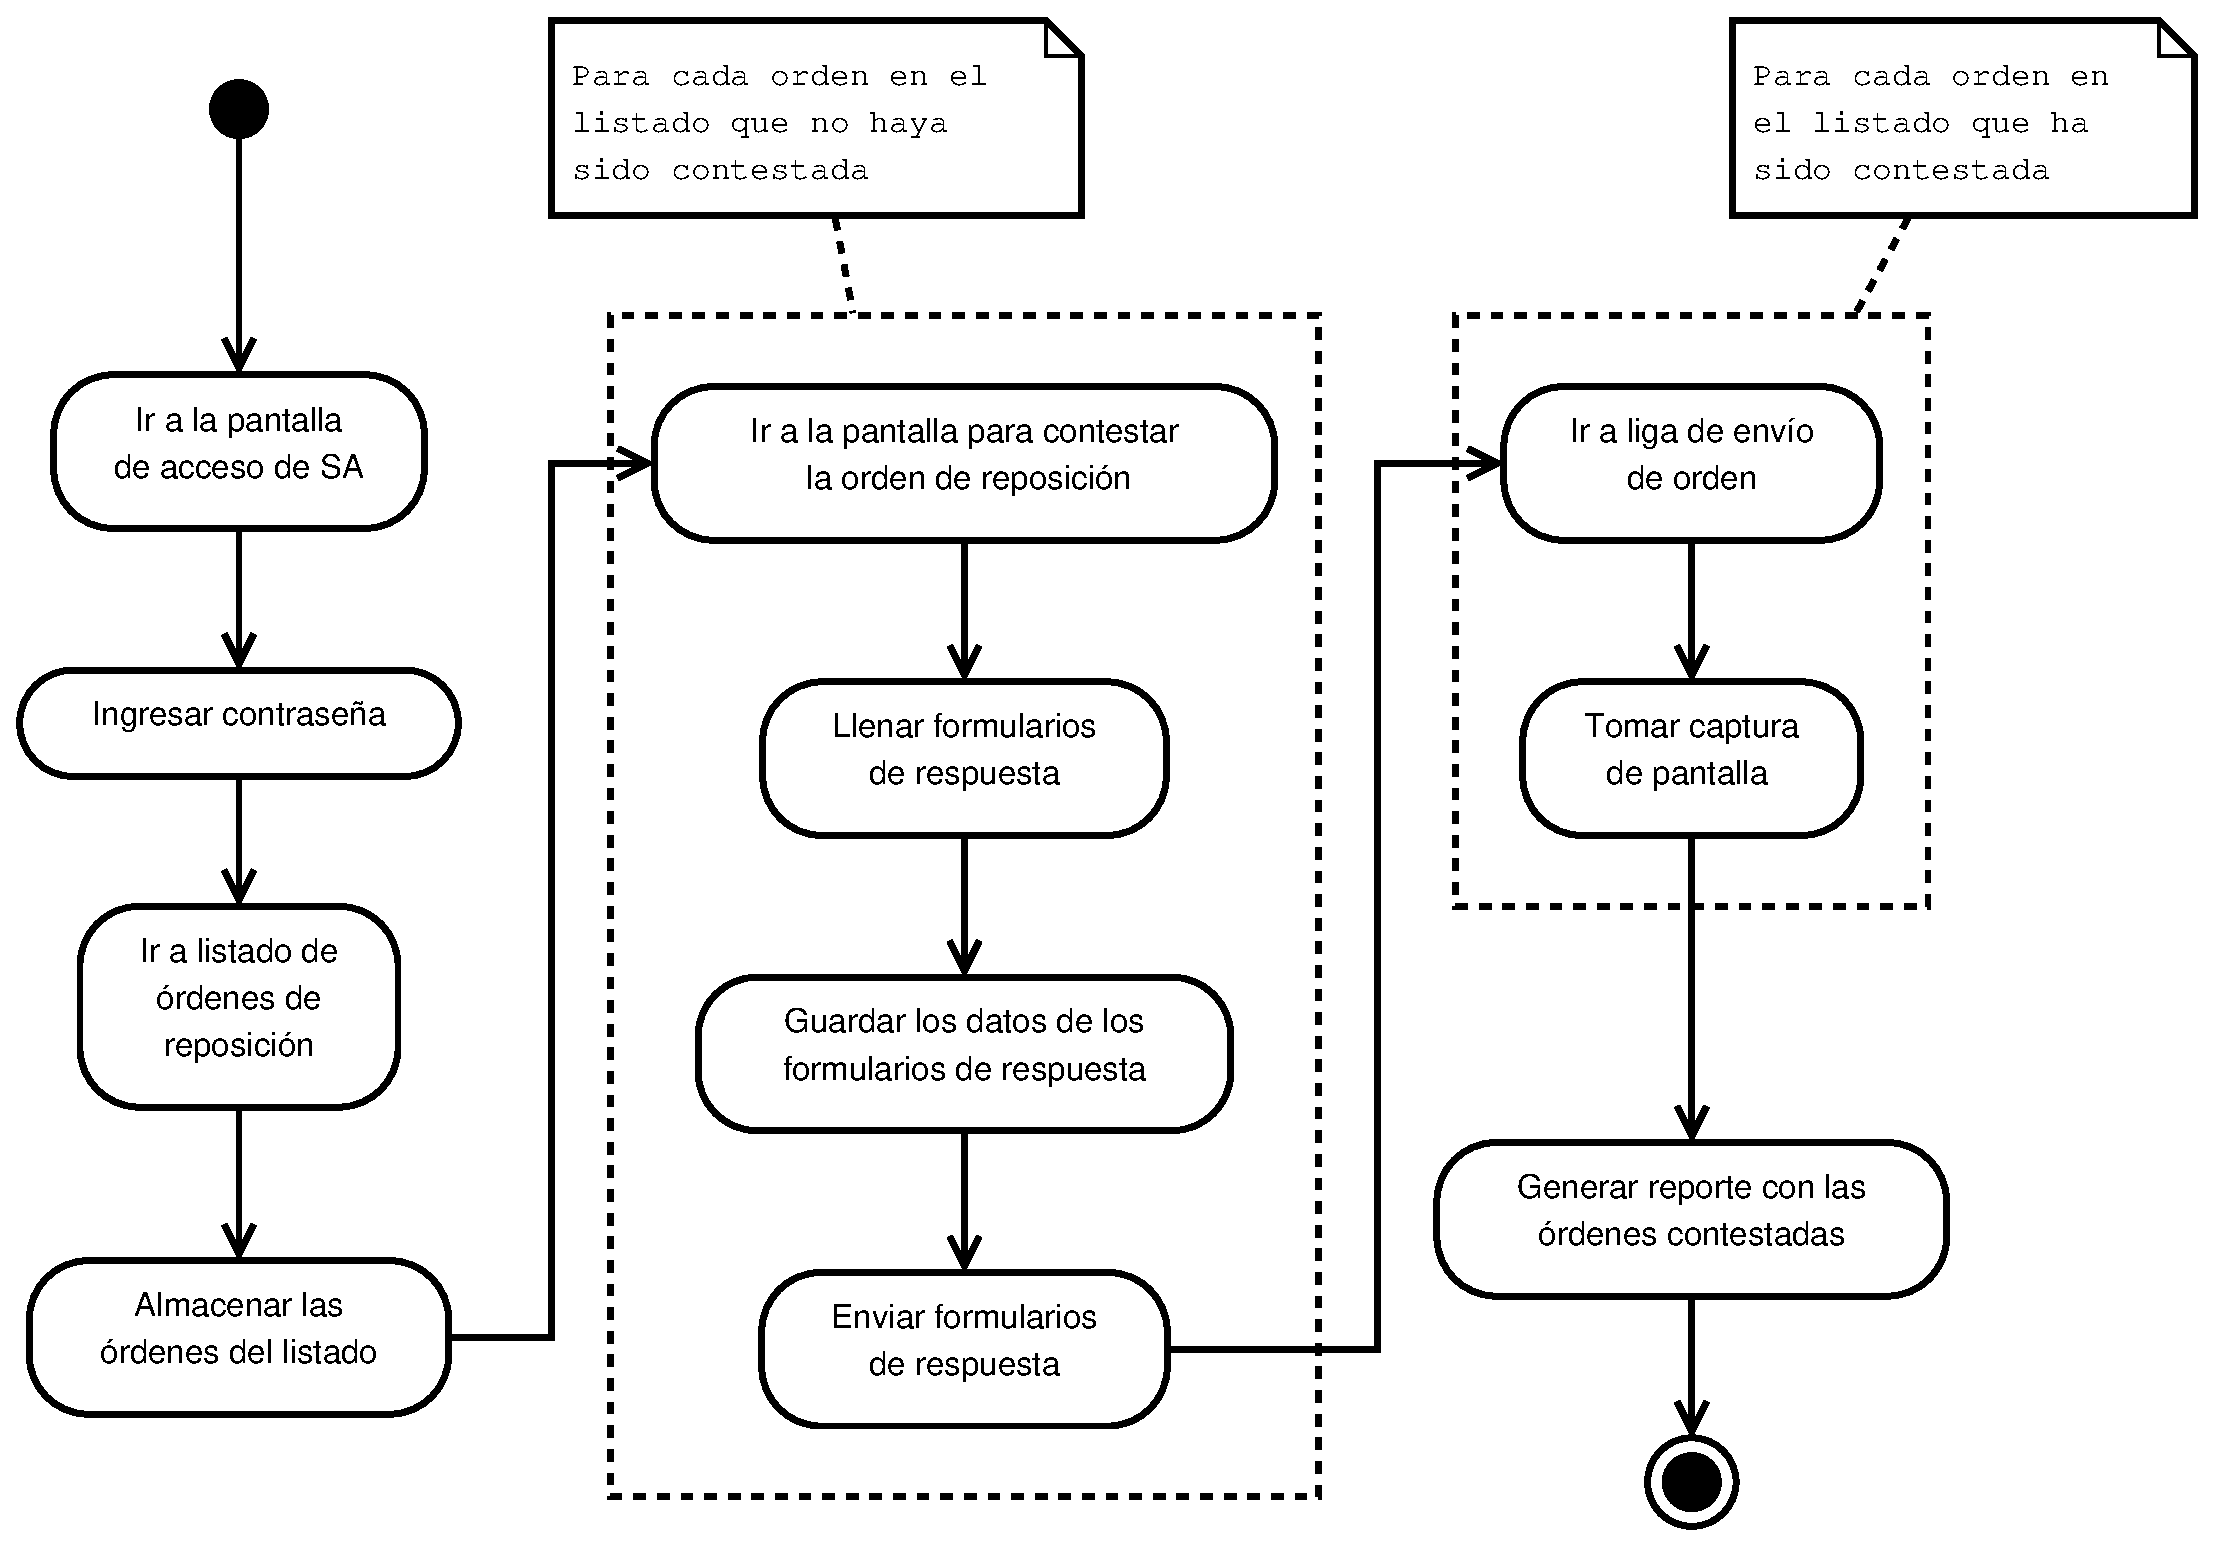
\includegraphics[scale=0.4]{dia-activity-contestar}
  \caption{Diagrama de proceso de negocio que sigue un operador de la farmacéutica para contestar órdenes de reposición.}
  \label{fig:dia-activity-contestar}
\end{figure}

\subsubsection{Automatización del proceso para cotejar órdenes de reposición canceladas}
Automatizar la interacción del operador de la farmacéutica para conocer las órdenes de reposición que han sido canceladas recientemente por el instituto, como se muestra en el diagrama de proceso de negocio en la Figura \ref{fig:dia-activity-verificar} \footnote{
Ver también la Figura \ref{fig:flow-proc-verificar}}.
\begin{figure}[h]
  \centering
  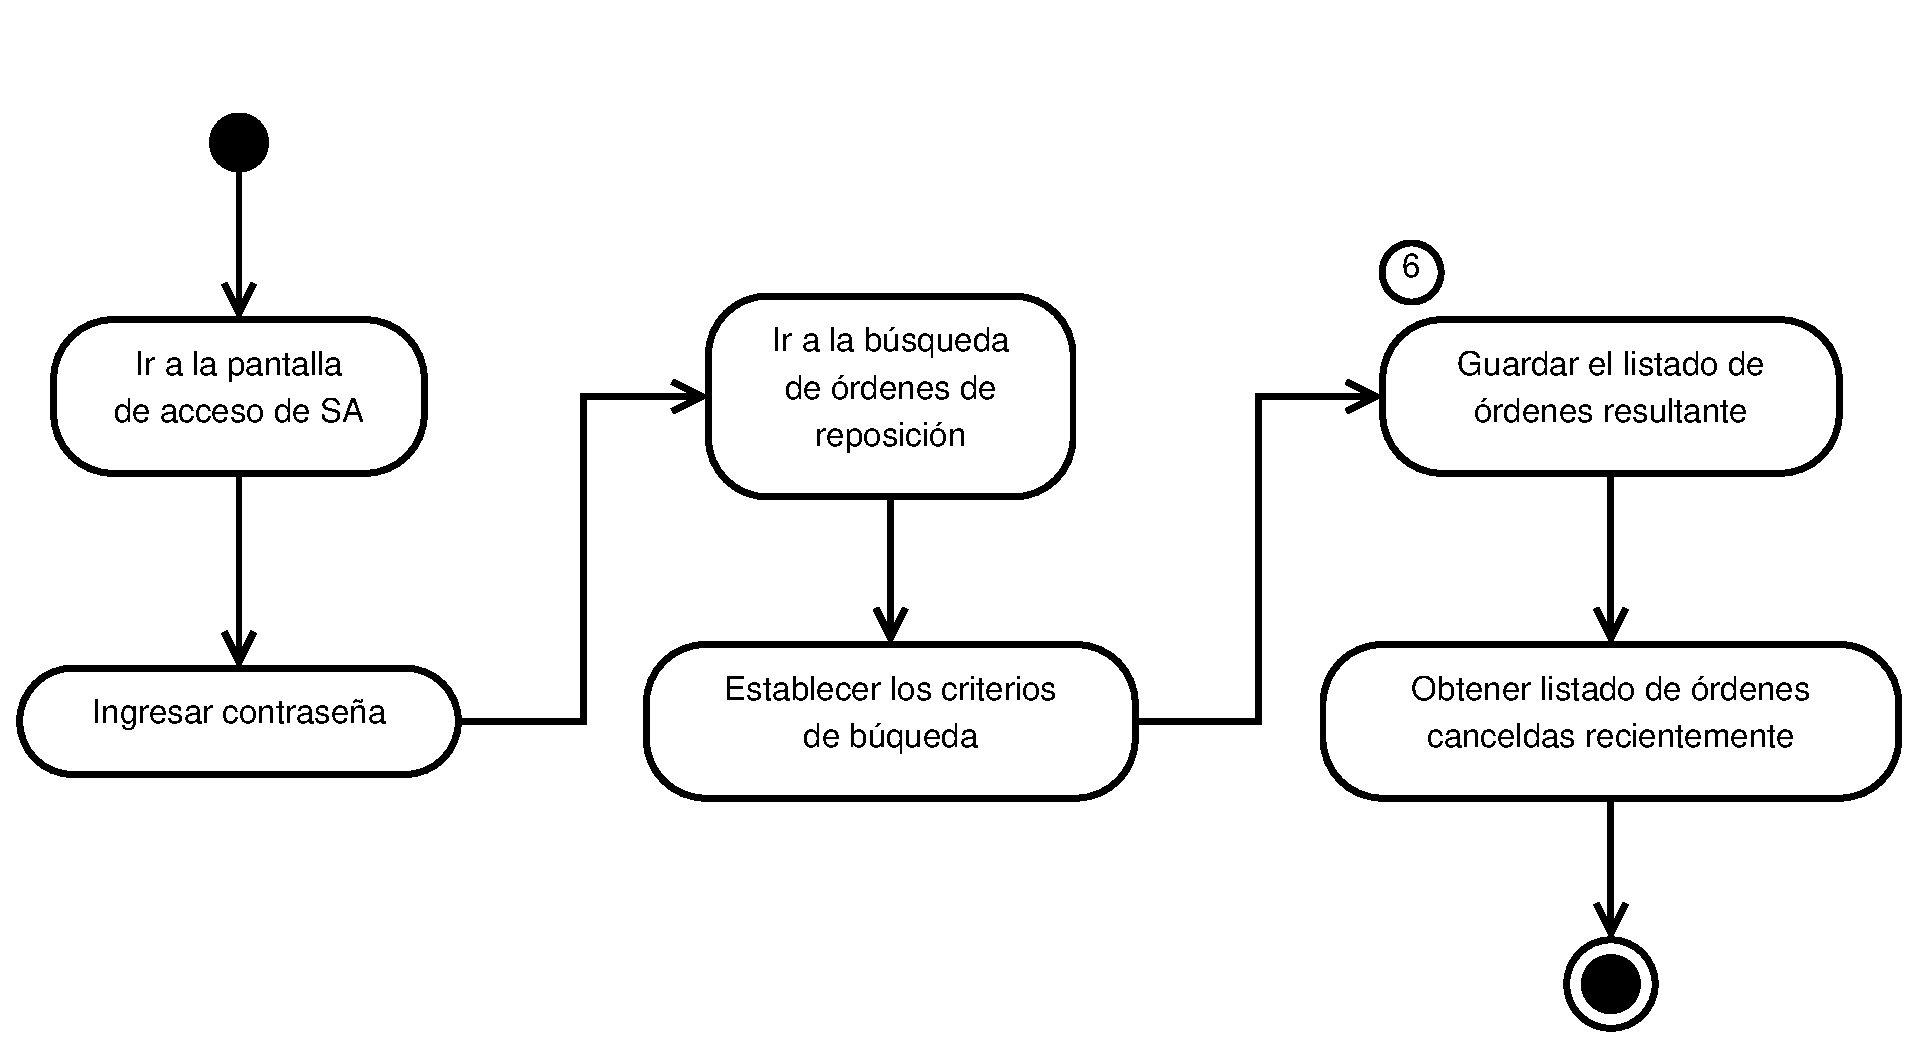
\includegraphics[scale=0.4]{dia-activity-verificar}
  \caption{Diagrama de proceso de negocio que sigue un operador de la farmacéutica para verificar órdenes de reposición canceladas.}
  \label{fig:dia-activity-verificar}
\end{figure}

\subsubsection{Interfaz WEB para la administración de órdenes de reposición contestadas}
Todos los requerimientos de administración de órdenes de reposición y generación de reportes deben ser accedidos mediante una interfaz web protegida por nombre de usuario y contraseña\footnote{Excepto lo referente a los procesos automatizados de los operadores de la farmacéutica}, como se muestra en la Figura \ref{fig:maq-login}.
\begin{figure}[h]
  \centering
  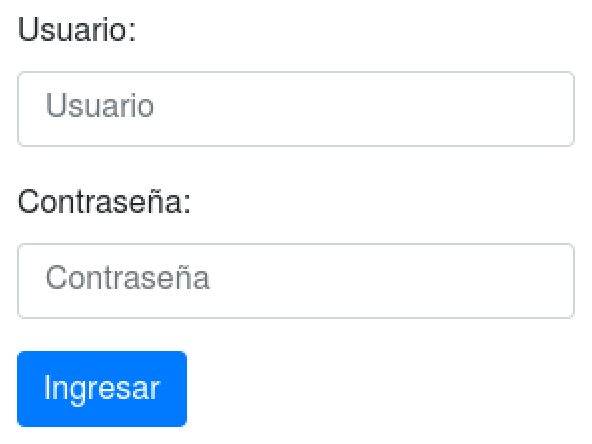
\includegraphics[scale=0.5]{maq-login} 
  \caption{Maqueta del acceso a la interfaz web.}
  \label{fig:maq-login}
\end{figure} 

\subsubsection{Búsqueda de órdenes de reposición}
En la interfaz web existe la posibilidad de buscar entre las órdenes de reposición contestadas mediante el número de orden de reposición. Esta opción entrega solo una orden de reposición, o bien se puede utilizar un intervalo de fechas entre las cuales fueron atendidas tales órdenes, entregando un listado de todas las órdenes de reposición que fueron respondidas en dicho intervalo. Las órdenes resultantes de la búsqueda deben ofrecer la opción para visualizar la información almacenada durante el proceso de respuesta, como se muestra en la Figura \ref{fig:maq-search}
\begin{figure}[h]
  \centering
  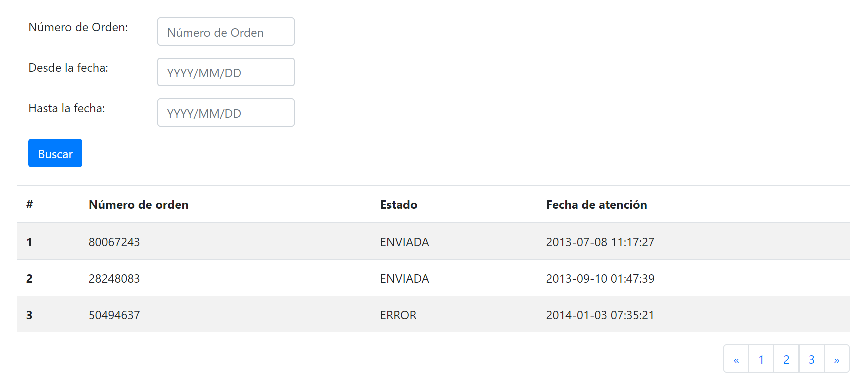
\includegraphics[width=\textwidth]{maq-search} 
  \caption{Maqueta de la búsqueda de órdenes.}
  \label{fig:maq-search}
\end{figure} 

\subsubsection{Visualización de orden de reposición}
La interfaz WEB tiene una sección donde se muestra el contenido de una orden de reposición almacenada en la base de datos (ver Figura \ref{fig:maq-crud}), esta vista es individual, (no es posible mostrar el contenido de más de una orden de reposición), además ofrece las opciones para modificar los datos de la orden (ver requerimiento \ref{req-edicion}) y para generar el acuse de envío.
\begin{figure}[h]
  \centering
  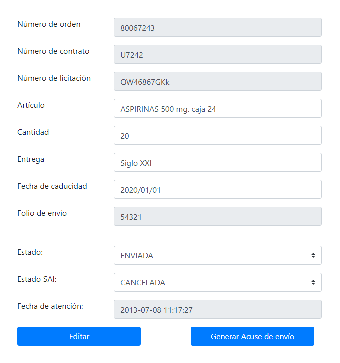
\includegraphics[scale=1]{maq-crud} 
  \caption{Maqueta del formulario para ver la información de una orden de reposición.}
  \label{fig:maq-crud}
\end{figure} 

\subsubsection{Edición de órdenes de reposición}\label{req-edicion}
La interfaz web cuenta con una vista (similar a la forma de mostrar la información de una orden de reposición) que permite la modificación de una orden de reposición (ver Figura \ref{fig:maq-crud}), esta vista es única (no es posible modificar más de una orden de reposición), así mismo no es posible modificar datos el número de orden y fecha de atención.

\subsubsection{Generación de reporte de órdenes de reposición contestadas}
El reporte con órdenes de reposición contestadas es acotado entre un par de fechas (con precisión de horas), tal reporte (ver Figura \ref{fig:maq-report}), como su nombre lo indica, contiene los números de orden de reposición y datos definidos por la farmacéutica\footnote{Por acuerdo de confidencialidad no se enunciarán los datos contenidos en los reportes.}
\begin{figure}[h]
  \centering
  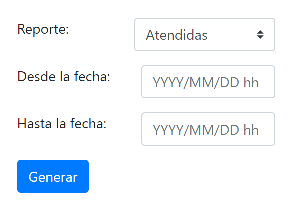
\includegraphics[scale=1.2]{maq-report} 
  \caption{Maqueta de la generación de reportes.}
  \label{fig:maq-report}
\end{figure} 

\subsubsection{Generación de formato de salida}
Este formato contiene los datos de las órdenes de reposición, las claves de los productos, como los nombres de los centros de salud. El reporte (ver Figura \ref{fig:maq-report})\footnote{Por acuerdo de confidencialidad no se enunciarán los datos contenidos en el formato de salida así como el contenido de los catálogos de claves de producto y centros de salud.} está acotado entre un par de fechas (con precisión de horas).

\subsubsection{Generación de reporte con las órdenes de reposición canceladas recientemente}
Genera un reporte con las órdenes de reposición canceladas recientemente (ver Figura \ref{fig:maq-report}), es decir, las órdenes de reposición que tienen el estado de “cancelada” y no se han marcado como canceladas en el proceso de respuesta.

\subsubsection{Actualización de catálogos}
Cargar de forma masiva, mediante un archivo separado por comas (ver Figura \ref{fig:maq-upload}), los catálogos con claves de medicamentos, centros de salud y claves propias del manejo de la farmaceútica. Los catálogos definidos para la operación del sistema AutoSA no podrán ser actualizados, por ejemplo, los catálogos que contienen los estados posibles de una orden de reposición cuando dentro del flujo de atención (ver Figura \ref{fig:dia-estados-orden}).
\begin{figure}[h]
  \centering
  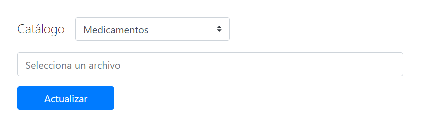
\includegraphics[scale=1.3]{maq-upload}
  \caption{Maqueta para la actualización de catálogos}
  \label{fig:maq-upload}
\end{figure}

\subsubsection{Actualización de estatus de órdenes de reposición canceladas}
Para realizar la actualización del estatus de las órdenes de reposición canceladas, el usuario carga al sistema un archivo de texto separado por comas, similar a la actualización de catálogos (ver Figura \ref{fig:dia-estados-orden}), con los números de las órdenes de reposición que han sido canceladas y se ha notificado al área correspondiente de la farmacéutica para cancelar la atención de dichas órdenes.

\subsection{Navegación dentro de la interfaz web}
La interfaz web muestra en todo momento un menú que permite la navegación entre las siguientes secciones (ver Figura \ref{fig:dia-nav-flow}):
\begin{enumerate}
  \item Generación de reportes
  \item Actualización de catálogos (incluye la actualización de órdenes canceladas).
  \item Búsqueda de órdenes de reposición
\end{enumerate}
\begin{figure}[h]
  \centering
  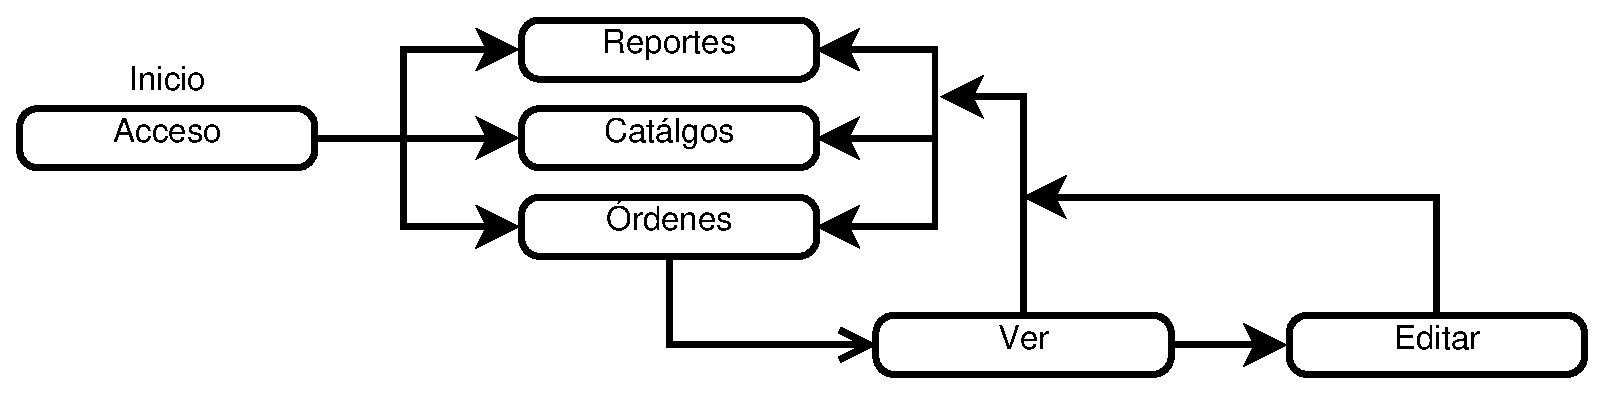
\includegraphics[scale=0.5]{dia-nav-flow}
  \caption{Mapa de navegación en la interfaz Web}
  \label{fig:dia-nav-flow}
\end{figure}


\subsection{Requerimientos no funcionales}\label{sec:nonfunctional-req}
El cliente ha solicitado que el proyecto se apegue a su infraestructura, para conservar el acuerdo de confidencialidad y evitar exponer al cliente a riesgos de seguridad informática por lo que el sistema debe de contar con un\footnote{Por políticas de seguridad de la farmacéutica no se enunciarán las herramientas e infraestructura utilizada, así como las versiones de las mismas}:
\begin{enumerate}
\item Sistema operativo capaz de ejecutar el software Java Virtual Machine (JVM).
\item Base de datos relacional SQL.
\item Uso de la herramienta Sahi para automatizar interacción con Sistema de Abastecimiento.
\item Las contraseñas de los usuarios para el acceso a la interfaz web deben ser almacenadas utilizando un algoritmo de cifrado.
\end{enumerate}


%===============================================================================
%===============================================================================


\section{Casos de uso}
Un caso de uso es la representación de las posibles interacciones entre el sistema y sus actores, entendiendo un actor como una instancia (usuario u otro sistema). Así mismo, un caso de uso describe la funcionalidad del sistema por medio de mensajes y respuestas entre el actor y el sistema\cite{ApressSE}. A continuación se muestra el diagrama de casos de uso del sistema AutoSA.

\begin{figure}[h]
  \centering
  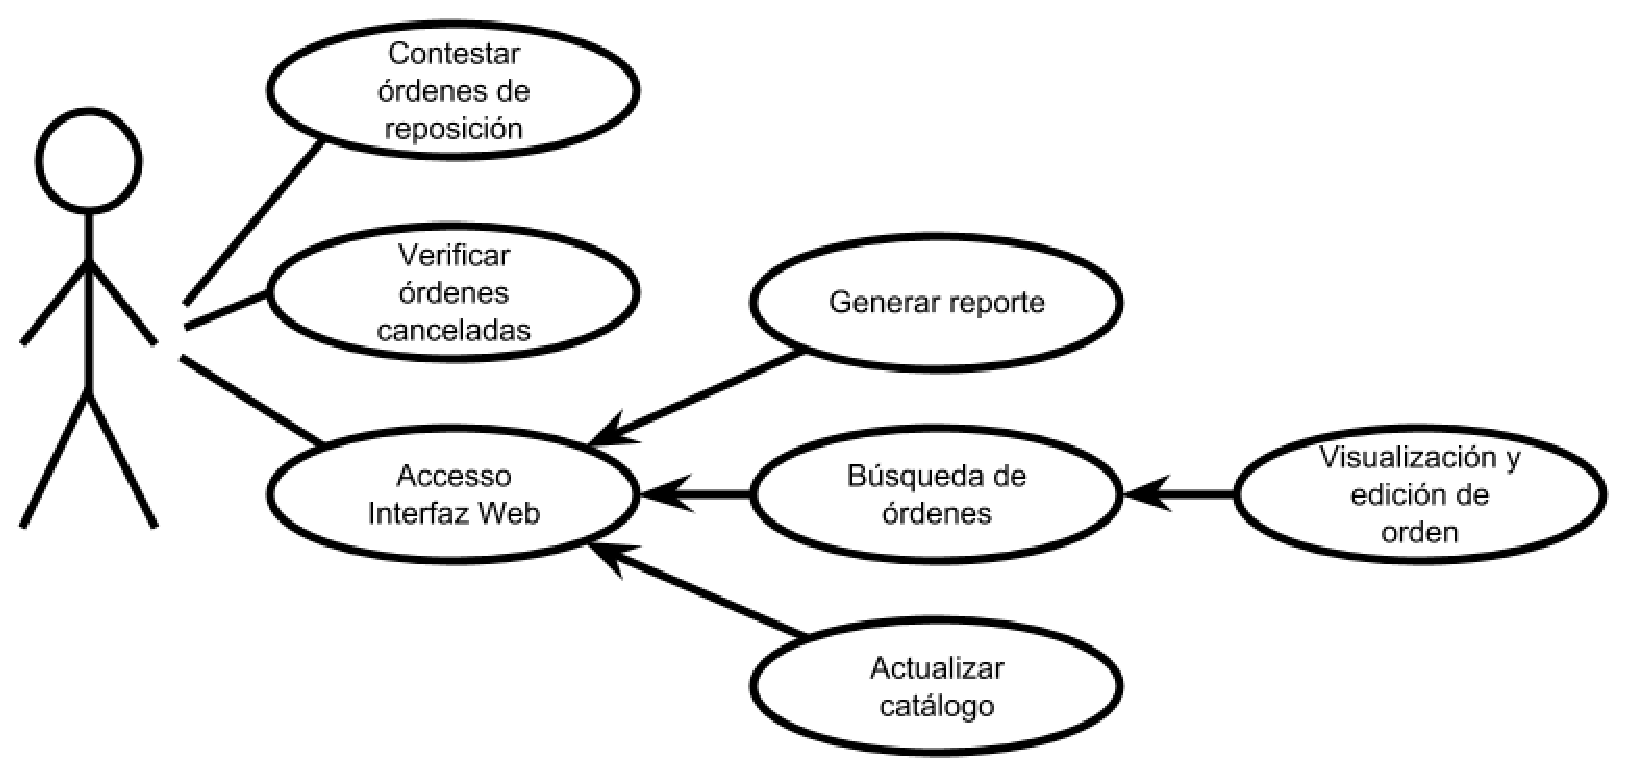
\includegraphics[width=\textwidth]{dia-casos-uso} 
  \caption{Diagrama de casos de uso.}
  \label{fig:dia-casos-uso}
\end{figure}

Con el fin de explicar mejor el flujo de atención de una orden de reposición es necesario mostrar el diagrama de estados de una orden de reposición durante el flujo de \textbf{envío de órdenes de reposición} (ver sección \ref{sec:intro-contexto}). Los estados que puede tomar una orden (ver Figura \ref{fig:dia-estados-orden}) indican:
\begin{itemize}
  \item Si la solicitud está lista para ser procesada: \textbf{Nueva}, \textbf{Contestada}.
  \item Si está siendo procesada: \textbf{Siendo Contestada}, \textbf{Siendo Enviada}.
  \item Si ha terminado el ciclo correctamente: \textbf{Enviada}.
  \item Si ha terminado el ciclo con errores: \textbf{Error}.
\end{itemize} 

\begin{figure}[h]
  \centering
  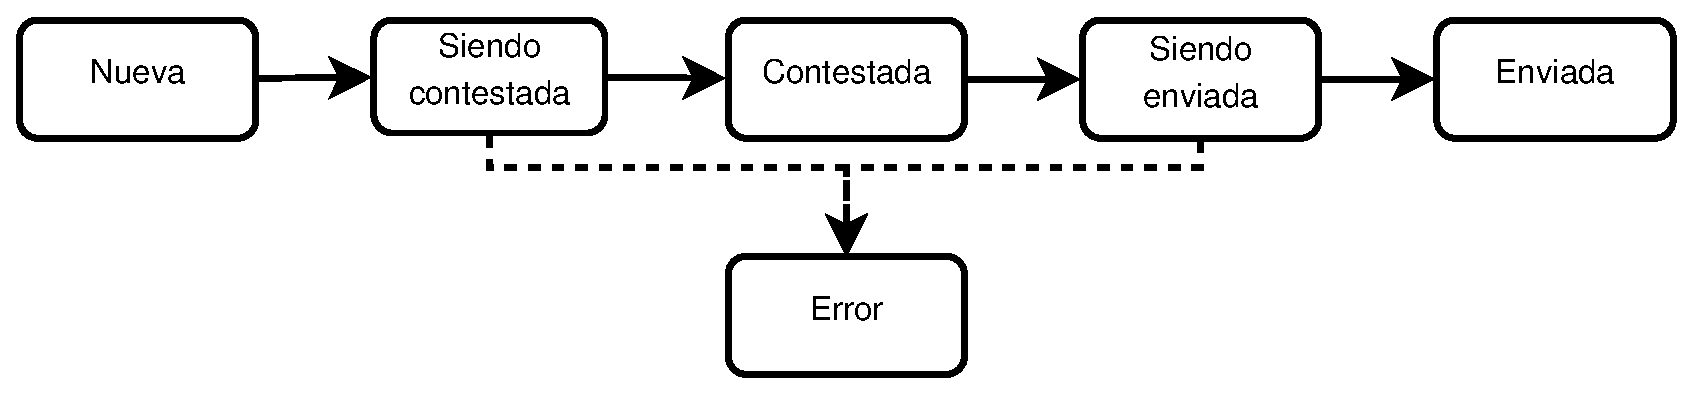
\includegraphics[width=\textwidth]{dia-estados-orden} 
  \caption{Diagrama de estados de una orden de reposición durante la ruta de respuesta de órdenes de reposición.}
  \label{fig:dia-estados-orden}
\end{figure}

Es importante mencionar que en las siguientes descripciones de caso de uso no se hará referencia al contenido exacto de las páginas así como el nombre de los campos, únicamente se hará mención de los campos necesarios para dar una explicación clara del caso.

\subsection{Contestar órdenes}\label{cu-contestar}
\paragraph{Identificador:}
CU-CONTESTAR
\paragraph{Actores:}
Usuario
\paragraph{Descripción:}
El procedimiento completo para contestar las órdenes de reposición listadas en el Sistema de Abastecimiento del instituto (ver Figura \ref{fig:dia-activity-contestar}), el alcance de este caso comprende el acceso al Sistema de Abastecimiento, contestar y enviar las órdenes de reproducción almacenando los datos y generando la captura de pantalla de dichas órdenes.\\
Queda fuera de alcance la obtención del reporte con las órdenes de reposición que han sido canceladas recientemente es cubierto por el caso de uso Generación de Reportes.
\paragraph{Precondiciones:}
\begin{enumerate}
  \item El Sistema de Abastecimiento se encuentra funcionando correctamente.
  \item El usuario cuenta con las credenciales para ingresar al Sistema de Abastecimiento.
\end{enumerate}
\paragraph{Secuencia normal:}
\begin{enumerate}
  \item Inicia sesión en Sistema de Abastecimiento: provee nombre de usuario y le solicita al usuario ingresar la contraseña.
  \item Dirige el explorador a la pantalla donde se encuentra el listado con las órdenes de reposición que no han sido contestadas.
  \item Para cada orden de reposición del listado que se muestra se aplica el caso de uso CU-GUARDAR-NUEVA.
  \item Para cada solicitud en la base de datos con estado \textbf{Nueva} se aplican los casos de uso:
  \begin{enumerate}
    \item CU-RESPONDER-ORDEN.
  \end{enumerate}
  \item Para cada solicitud con estatus \textbf{Contestada}:
  \begin{enumerate}
    \item CU-ENVIAR-ORDEN
    \item CU-GENERAR-ACUSE
  \end{enumerate}
  \item El programa se repite desde el paso 2 hasta terminar las solicitudes sin contar las marcadas con estatus \textbf{Error}.
  \item Registra el fin del procedimiento en la base de datos.
\end{enumerate}
\paragraph{Postcondiciones:}
\begin{enumerate}
  \item Todas las órdenes de reposición listadas han sido contestadas y enviadas.
  \item Se han registrado todas las órdenes de reposición atendidas en la base de datos.
  \item Los acuses de envió de las órdenes de reposición se encuentran en el sistema de archivos.
\end{enumerate}
\paragraph{Excepciones:}
\begin{enumerate}
  \item Si en algún momento se detecta la pérdida de sesión en la página Sistema de Abastecimiento, se reinicia el procedimiento desde el paso 1 de este caso de uso.
  \item Cualquier error durante la ejecución de este caso de uso será registrado en la bitácora el sistema.
\end{enumerate}


\subsection{Guardar nueva orden}\label{cu-guardar-nueva}
\paragraph{Identificador:}
CU-GUARDAR-NUEVA
\paragraph{Actores:}
Robot
\paragraph{Descripción:}
Una orden de reposición es almacenada por primera vez con la información que se muestra en el listado de órdenes de reposición.
\paragraph{Precondiciones:}
\begin{enumerate}
  \item Se tiene indicado un renglón del listado de órdenes de reposición sobre el cuál se realizará este caso de uso.
\end{enumerate}
\paragraph{Secuencia normal:}
\begin{enumerate}
  \item Del listado de órdenes de reposición, cada solicitud es ingresada a la base de datos con estatus \textbf{Nueva} y datos provenientes del listado:
  \begin{enumerate}
    \item Contrato.
    \item Solicitud.
    \item Número de orden.
    \item Fecha de expedición.
    \item Almacén destino.
    \item \textit{URL} de respuesta.
    \item \textit{URL} de envío: generada reemplazando el parámetro en la \textit{URL} de respuesta ``responde'' por ``envia''\footnote{Dado que es una palabra en una URL no es recomendable el uso de acentos, por lo tanto se escribe \textbf{envia} y no \textbf{envía}}.
  \end{enumerate}
\end{enumerate}
\paragraph{Postcondiciones:}
\begin{enumerate}
  \item La orden de reposición se encuentra almacenada en la base de datos.
\end{enumerate}
\paragraph{Excepciones:}
\begin{enumerate}
  \item Si el listado muestra la URL de envío y la orden no ha sido almacenada, entonces la orden es almacenada con estado \textbf{Contestada} y se registra la \textbf{cantidad solicitada} en 0.
  \item Si ocurre algún error la orden es almacenada con estado \textbf{Error}.
\end{enumerate}


\subsection{Responder orden}\label{cu-responder-orden}
\paragraph{Identificador:}\label{cu-responder-orden}
CU-RESPONDER-ORDEN
\paragraph{Actores:}
Robot
\paragraph{Descripción:}
En la pantalla para contestar una orden de reposición se llenan los formularios y se almacena la información de la pantalla en el registro de la base de datos que corresponde a la orden de reposición.
\paragraph{Precondiciones:}
\begin{enumerate}
  \item Se indica una orden de reposición almacenada en la base de datos sobre la cual se aplica este caso de uso.
  \item La orden de reposición se encuentra almacenada en la base de datos.
  \item La orden de reposición tiene estado \textbf{Nueva}.
\end{enumerate}
\paragraph{Secuencia normal:}
\begin{enumerate}
  \item Cambia el estado de la orden a \textbf{Siendo Contestada}.
  \item Dirige el explorador a la \textit{URL} de respuesta (ver caso de uso CU-GUARDAR-NUEVA).
  \item Llena el formulario que se presenta en esta pantalla con las siguientes consideraciones:
  \begin{enumerate}
    \item Fecha de fabricación: primer día del año en curso si la fecha actual no es del mes de diciembre, en caso contrario se toma el año siguiente.
    \item Fecha de caducidad: último día del año en curso si la fecha actual no es del mes de diciembre, en caso contrario se toma el año siguiente.
  \end{enumerate}
  \item Almacena en la base de datos los campos de los formularios.
  \item Activar el botón ``contestar'' del formulario de la orden de reposición.
  \item Cambia el estado de la orden a \textbf{Contestada}.
\end{enumerate}
\paragraph{Postcondiciones:}
\begin{enumerate}
  \item Los formularios de la pantalla han sido completados correctamente.
  \item Los datos del formulario se encuentran almacenado en la base de datos.
  \item El estado de la orden en la base de datos es \textbf{Contestada}.
\end{enumerate}
\paragraph{Excepciones:}
\begin{enumerate}
  \item Si ocurre algún error la orden es almacenada con estado \textbf{Error}.
\end{enumerate}


\subsection{Enviar orden}\label{cu-enviar-orden}
\paragraph{Identificador:}
CU-ENVIAR-ORDEN
\paragraph{Actores:}
Robot
\paragraph{Descripción:}
Enviar la orden de reposición contestada de regreso al Sistema de Abastecimiento.
\paragraph{Precondiciones:}
\begin{enumerate}
  \item Una orden de reposición registrada en la base de datos.
  \item La orden de reposición tiene estado \textbf{Contestada}.
\end{enumerate}
\paragraph{Secuencia normal:}
\begin{enumerate}
  \item Cambia estado de la orden a \textbf{Siendo Enviada}.
  \item El explorador dirige a la \textit{URL de envío}.
  \item Guardar el folio de envío en la base de datos.
  \item Cambia estado de la orden a \textbf{Enviada}.
\end{enumerate}
\paragraph{Postcondiciones:}
\begin{enumerate}
  \item El folio de envió de la orden de reposición se encuentra guardado en la base datos.
  \item El estado de la orden en la base de datos es \textbf{Enviada}.
\end{enumerate}
\paragraph{Excepciones:}
\begin{enumerate}
  \item Si ocurre algún error la orden es almacenada con estado \textbf{Error}.
\end{enumerate}


\subsection{Generar acuse de envío}\label{cu-generar-acuse}
\paragraph{Identificador:}
CU-GENERAR-ACUSE
\paragraph{Actores:}
Robot
\paragraph{Descripción:}
Generar el acuse de envío de la orden de reposición.
\paragraph{Precondiciones:}
\begin{enumerate}
  \item Una orden de reposición registrada en la base de datos.
  \item La orden de reposición tiene estado \textbf{Enviada}.
\end{enumerate}
\paragraph{Secuencia normal:}
\begin{enumerate}
  \item Extraer la información de la orden de reposición de la base de datos.
  \item Mandar la generación del acuse de envío.
  \item Colocar el documento generado en el sistema de archivos.
\end{enumerate}
\paragraph{Postcondiciones:}
\begin{enumerate}
  \item Un documento en el sistema de archivos que contiene el acuse de envío.
\end{enumerate}
\paragraph{Excepciones:}
\begin{enumerate}
  \item En caso de algún error se registra el error en la bitácora del sistema (el usuario posteriormente podrá volver a imprimir el acuse, ver caso de uso CU-VISUALIZAR).
\end{enumerate}


\subsection{Verificar órdenes}\label{cu-verificar}
\paragraph{Identificador:}
CU-VERIFICAR
\paragraph{Actores:}
Usuario
\paragraph{Descripción:}
Modelar el procedimiento automatizado para verificar órdenes de reposición canceladas (ver Figura \ref{fig:dia-activity-verificar}), el alcance de este caso de uso comprende el acceso al Sistema de Abastecimiento, búsqueda de órdenes de reposición con estado \textbf{Cancelado} y comparación con la base de datos.\\
Queda fuera de alcance: la actualización masiva del estado de órdenes de reposición es cubierto en el caso de uso \textbf{CU-ACTUALIZAR-CATALOGO}; y la obtención del reporte con las órdenes de reposición que han sido canceladas recientemente es cubierto por el caso de uso \textbf{CU-GENERAR-REPORTE}.
\paragraph{Precondiciones:}
\begin{enumerate}
  \item El Sistema de Abastecimiento se encuentra funcionando correctamente.
  \item El usuario cuenta con las credenciales para ingresar al Sistema de Abastecimiento.
\end{enumerate}
\paragraph{Secuencia normal:}
\begin{enumerate}
  \item Inicia sesión en Sistema de Abastecimiento: provee nombre de usuario y le solicita al usuario ingresar la contraseña.
  \item Dirige el explorador a la pantalla de búsqueda de órdenes de reposición.
  \item Llena el formulario para el filtro de búsqueda:
  \begin{enumerate}
    \item Rango de fechas que comprende los últimos siete días desde la fecha actual.
    \item Estado \textbf{Cancelada}.
  \end{enumerate}
  \item Del listado de órdenes de reposición resultantes genera una lista con el número de orden de cada renglón.
  \item Con el listado del paso anterior se realiza el caso de uso \textbf{CU-ACTUALIZAR-ESTATUS-SA}.
\end{enumerate}
\paragraph{Postcondiciones:}
\begin{enumerate}
  \item Se cuenta con la relación de órdenes de reposición atendidas por el sistema que han sido canceladas en el Sistema de Abastecimiento y no se tenía conocimiento previo.
  \item Las órdenes de reposición publicadas en el Sistema de Abastecimiento dentro de los últimos siete día a la fecha actual reflejan en la base de datos dentro del campo \textbf{Estado Sistema de Abastecimiento} el estado de vigencia en el Sistema de Abastecimiento.
\end{enumerate}
\paragraph{Excepciones:}
\begin{enumerate}
  \item Cualquier error durante la ejecución de este caso de uso será registrado en la bitácora el sistema.
\end{enumerate}


\subsection{Actualizar estatus Sistema de Abastecimiento}\label{cu-actualizar-estatus-sa}
\paragraph{Identificador:}
CU-ACTUALIZAR-ESTATUS-SA
\paragraph{Actores:}
Robot
\paragraph{Descripción:}
Actualizar en forma masiva el estado de atención en el Sistema de Abastecimiento dentro de la base de datos del sistema AutoSA.
\paragraph{Precondiciones:}
\begin{enumerate}
  \item Se cuenta con una lista de órdenes de reposición.
  \item Las órdenes listadas tienen estado \textbf{Cancelada} en el Sistema de Abastecimiento. 
\end{enumerate}
\paragraph{Secuencia normal:}
\begin{enumerate}
  \item Actualiza el estado Sistema de Abastecimiento de las órdenes de reposición en la base de datos.
\end{enumerate}
\paragraph{Postcondiciones:}
\begin{enumerate}
  \item Las órdenes de reposición recibidas tienen estado \textbf{Cancelada} en el campo \textbf{Estado Sistema de Abastecimiento} dentro de la base de datos.
\end{enumerate}
\paragraph{Excepciones:}
\begin{enumerate}
  \item Las órdenes de reposición que no estén registradas en la base de datos se registrarán con campos nulos a excepción del número de orden.
  \item Cualquier error durante la ejecución de este caso de uso será registrado en la bitácora el sistema.
\end{enumerate}


\subsection{Entrar en interfaz Web}\label{cu-entrar-web}
\paragraph{Identificador:}
CU-ENTRAR-WEB
\paragraph{Actores:}
Usuario
\paragraph{Descripción:}
Explicar el flujo para autorizar la entrada de un usuario a la interfaz Web del sistema, como se muestra en diagrama de actividad de la Figura \ref{fig:dia-activity-login}, este es el punto de acceso que tienen los usuarios para hacer acciones de administración de las órdenes de reposición atendidas por las rutinas de automatización, generación de reportes y actualización de catálogos.
\begin{figure}[h]
  \centering
  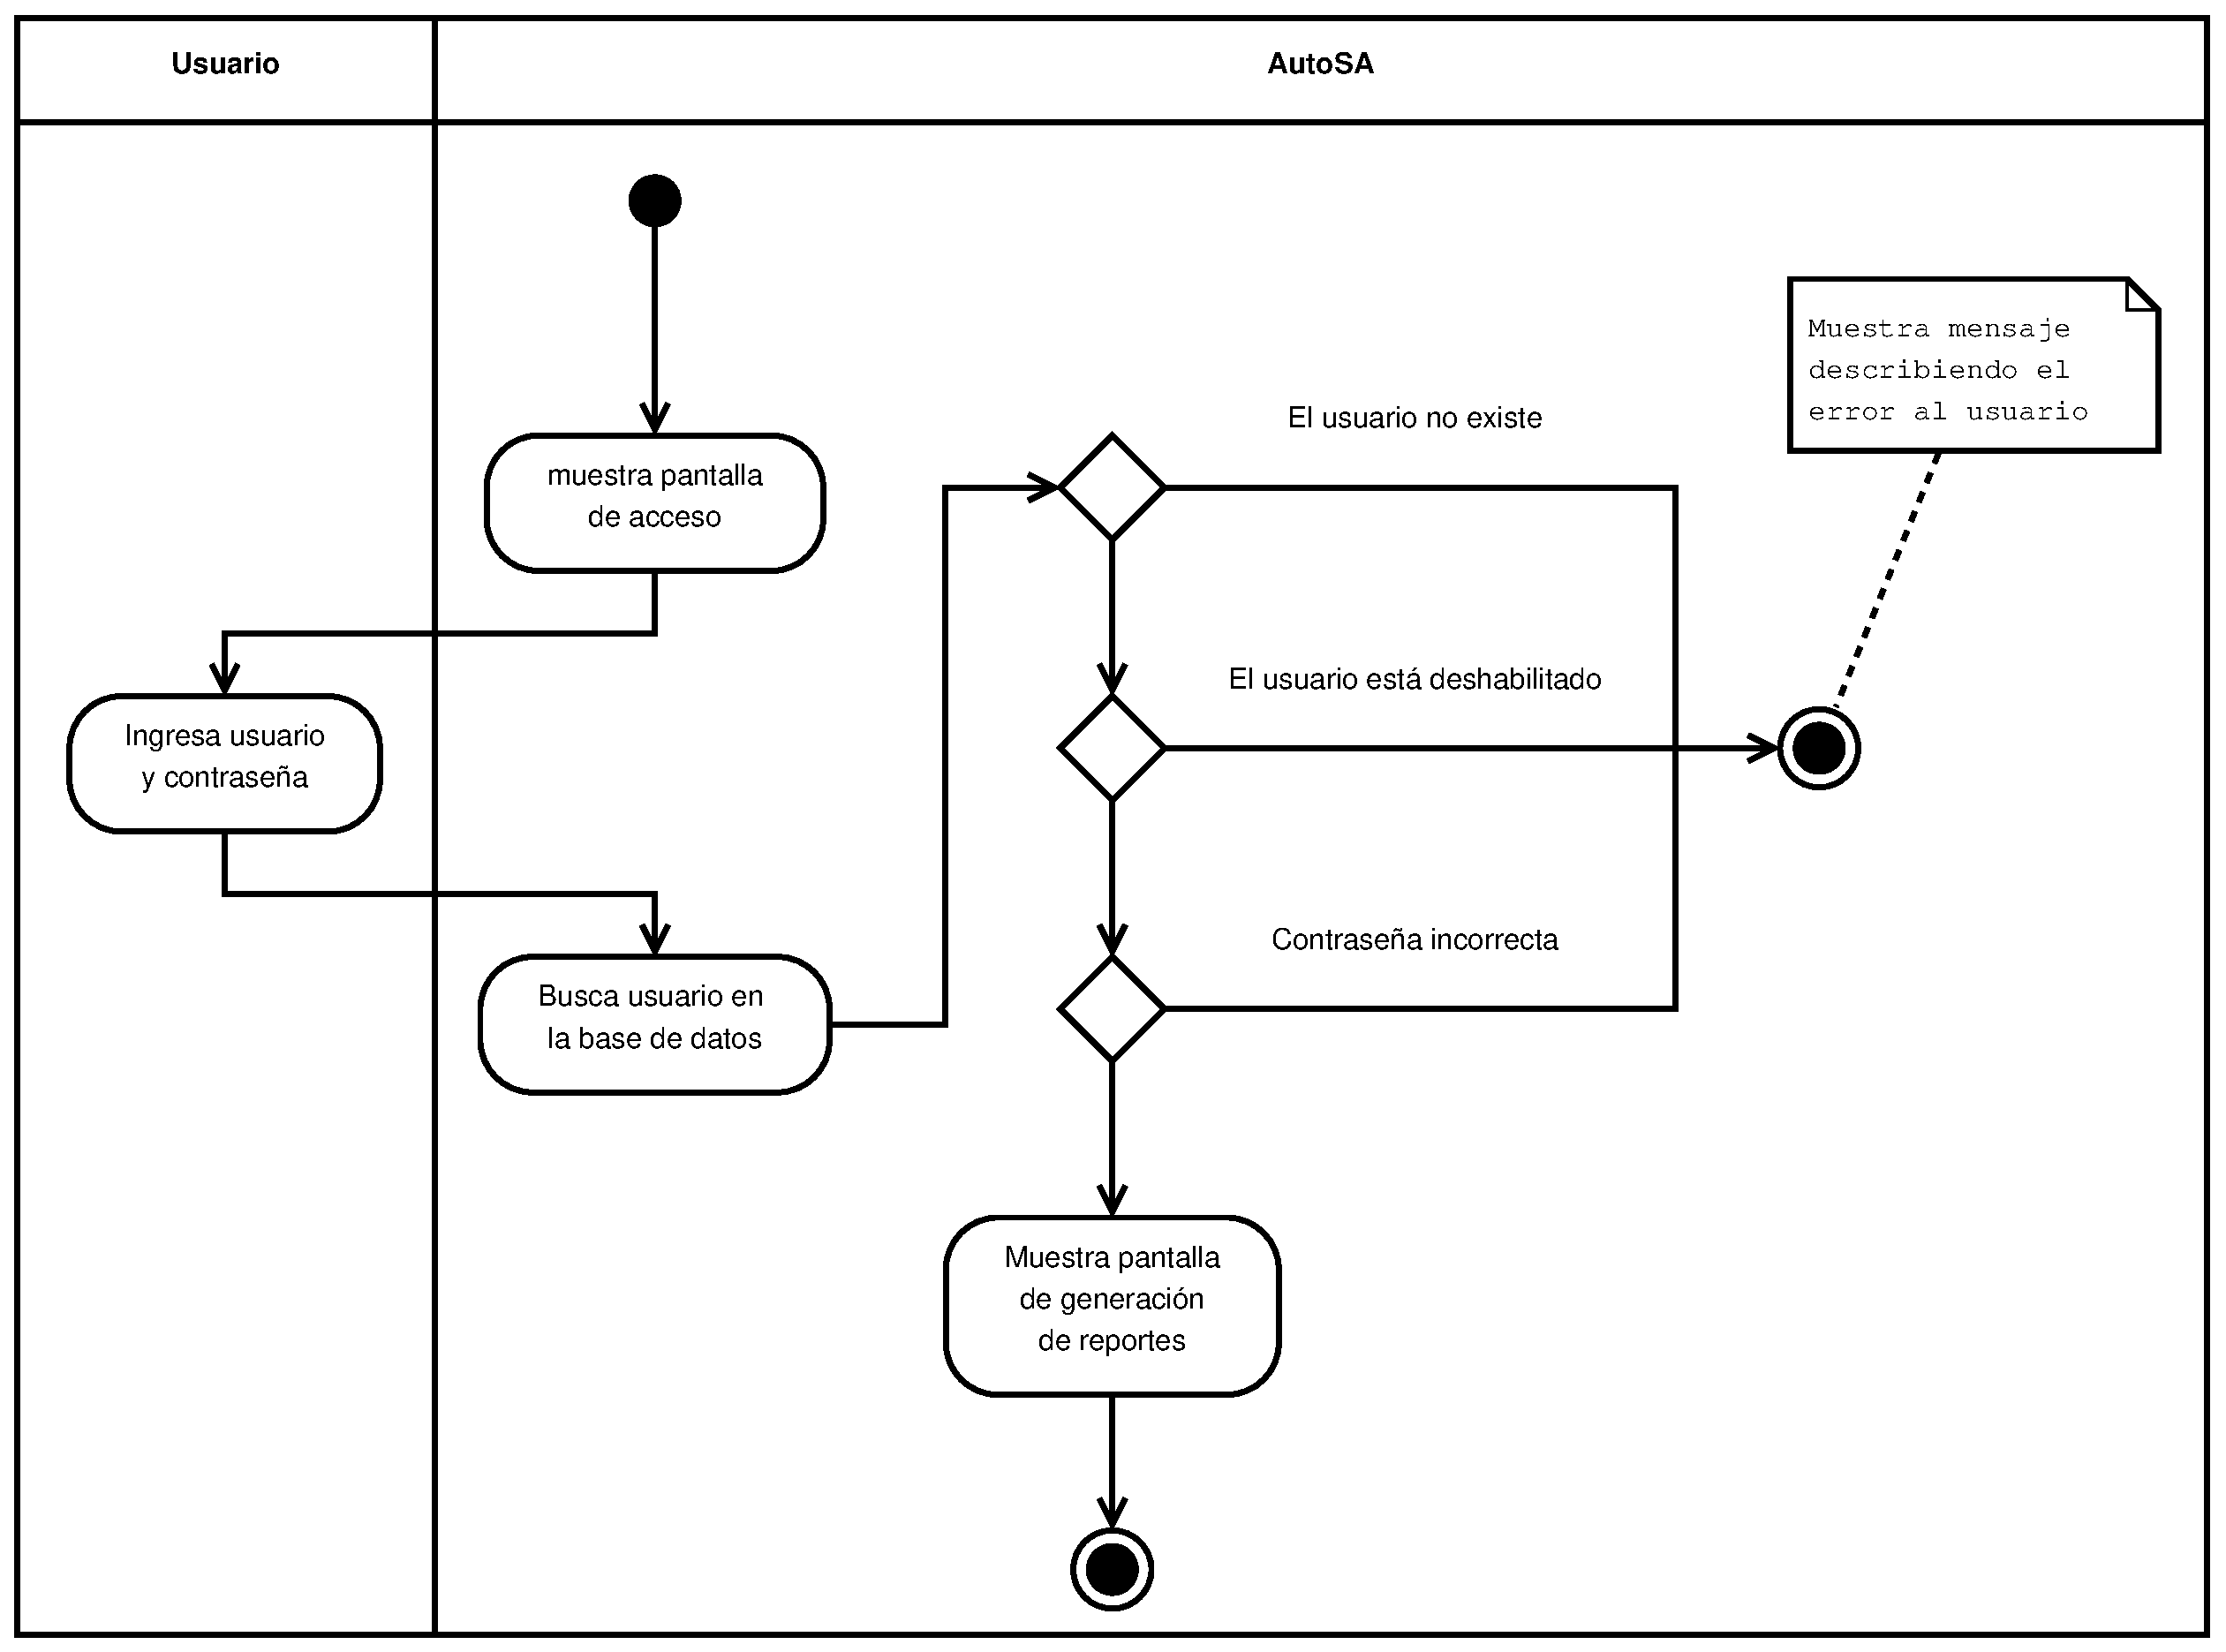
\includegraphics[width=\textwidth]{dia-activity-login}
  \caption{Diagrama de actividad del flujo de acceso al sistema.}
  \label{fig:dia-activity-login}
\end{figure}
\paragraph{Precondiciones:}
\begin{enumerate}
  \item El usuario se encuentra previamente registrado en el sistema.
  \item El usuario cuanta con credenciales vigentes para ingresar a la interfaz web.
\end{enumerate}
\paragraph{Secuencia normal:}
\begin{enumerate}
  \item El sistema muestra la pantalla de acceso.
  \item El usuario ingresa los campos:
  \begin{enumerate}
    \item Nombre de usuario.
    \item Contraseña.
  \end{enumerate}
  \item El sistema busca el nombre de usuario en la base de datos
  \item El sistema compara la contraseña provista por el usuario con el valor almacenado en la base de datos.
  \item Muestra la pantalla de generación de reportes.
\end{enumerate}
\paragraph{Postcondiciones:}
\begin{enumerate}
  \item El usuario cuenta con un código temporal de acceso a la interfaz web.
  \item Se muestra la pantalla de generación de reportes.
\end{enumerate}
\paragraph{Excepciones:}
\begin{enumerate}
  \item En los siguientes esceneracios se concideran un error de autencación.
  \begin{itemize}
    \item El usuario no existe en la base de datos.
    \item El usuario tiene estado \textbf{deshabilitado}.
    \item La contraseña proporcionada no coincide con la almacenada. 
  \end{itemize}
\end{enumerate}

\subsection{Generar reporte}\label{cu-generar-reporte}
\paragraph{Identificador:}
CU-GENERAR-REPORTE
\paragraph{Actores:}
Usuario
\paragraph{Descripción:}
Este caso de uso ofrece al usuario la generación de reportes, es decir, ejecutar una consulta a la base de datos y vaciar el resultado en un archivo, como se muestra en el diagrama de actividad de la Figura \ref{fig:dia-activity-reporter}. La consulta puede ser ejecutada sobre una o más tablas, es importante mencionar que existen catálogos con claves de productos y clientes que cambian constantemente, ver caso de uso \textbf{CU-ACTUALIZAR-CATALOGO}.
\begin{figure}[h]
  \centering
  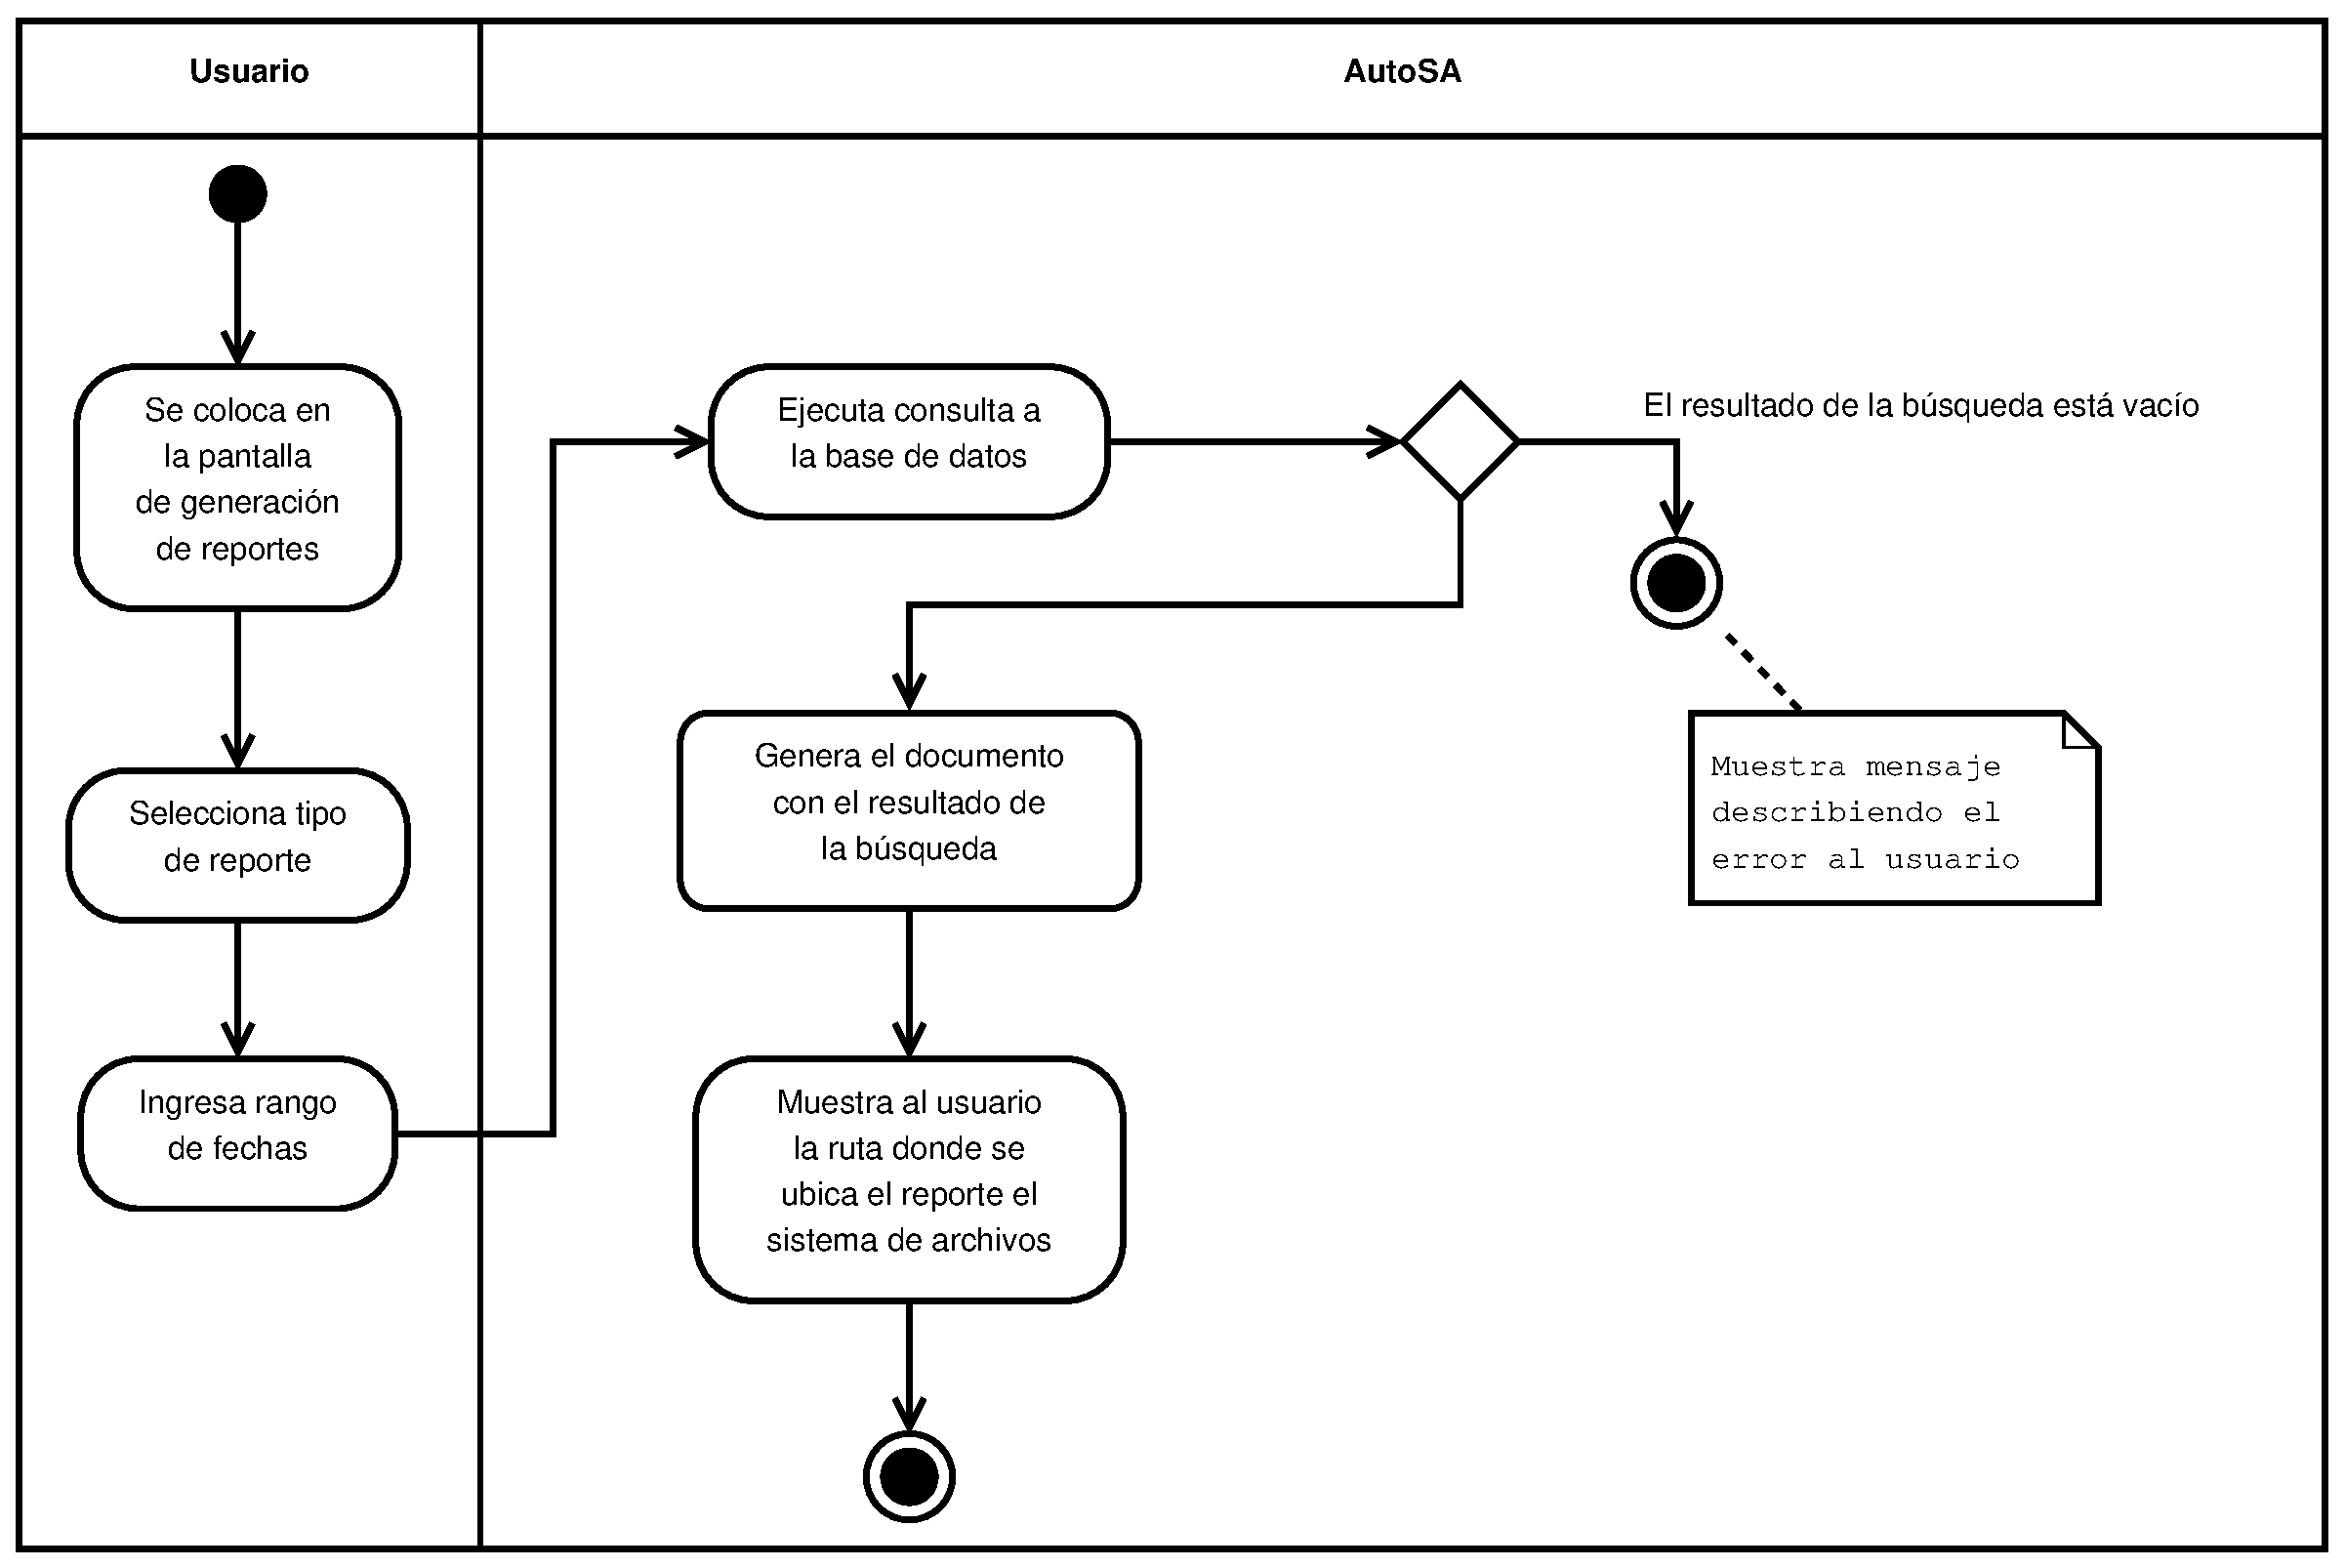
\includegraphics[width=\textwidth]{dia-activity-reporter}
  \caption{Diagrama de actividad del flujo para generación de reportes.}
  \label{fig:dia-activity-reporter}
\end{figure}
\paragraph{Precondiciones:}
\begin{enumerate}
  \item El usuario ha iniciado sesión correctamente en la interfaz web (ver caso de uso \textbf{CU-ENTRAR-WEB}).
\end{enumerate}
\paragraph{Secuencia normal:}
\begin{enumerate}
  \item El usuario navega a la pantalla de generación de reportes.
  \item En la pantalla de generación de reportes el usuario realiza las siguientes acciones:
    \begin{enumerate}
    \item Llenar el formulario de la pantalla con los siguientes campos:
    \begin{enumerate}
      \item \textbf{Tipo de reporte}
      \item \textbf{Fecha y hora inicial}
      \item \textbf{Fecha y hora final}
    \end{enumerate}
    \item Enviar el formulario.
  \end{enumerate}
  \item El sistema ejecuta los siguientes pasos:
  \begin{enumerate}
    \item Realiza para consulta a la base de datos definida para el reporte requerido en 1.a.
    \item El resultado del paso anterior es escrito en un archivo extendido de Excel y depositado en el sistema de archivos.
    \item Muestra al usuario la ruta en el sistema de archivos donde fue depositado el reporte.
  \end{enumerate}
\end{enumerate}
\paragraph{Postcondiciones:}
\begin{enumerate}
  \item El reporte se encuentra en el sistema de archivos dentro un archivo con formato extendido de Excel.
\end{enumerate}
\paragraph{Excepciones:}
\begin{enumerate}
  \item Si el reporte no cuenta con registros el archivo no se genera y se muestra un mensaje al usuario indicando la situación.
\end{enumerate}


\subsection{Actualizar catálogo}\label{cu-actualizar-catalogo}
\paragraph{Identificador:}
CU-ACTUALIZAR-CATALOGO
\paragraph{Actores:}
Usuario
\paragraph{Descripción:}
Define la actualización masiva de los catálogos en la base de datos mediante un archivo ingresado por un usuario de la interfaz Web, la Figura \ref{fig:dia-activity-cat-update} muestra el diagrama de actividad para este caso de uso.
\begin{figure}[h]
  \centering
  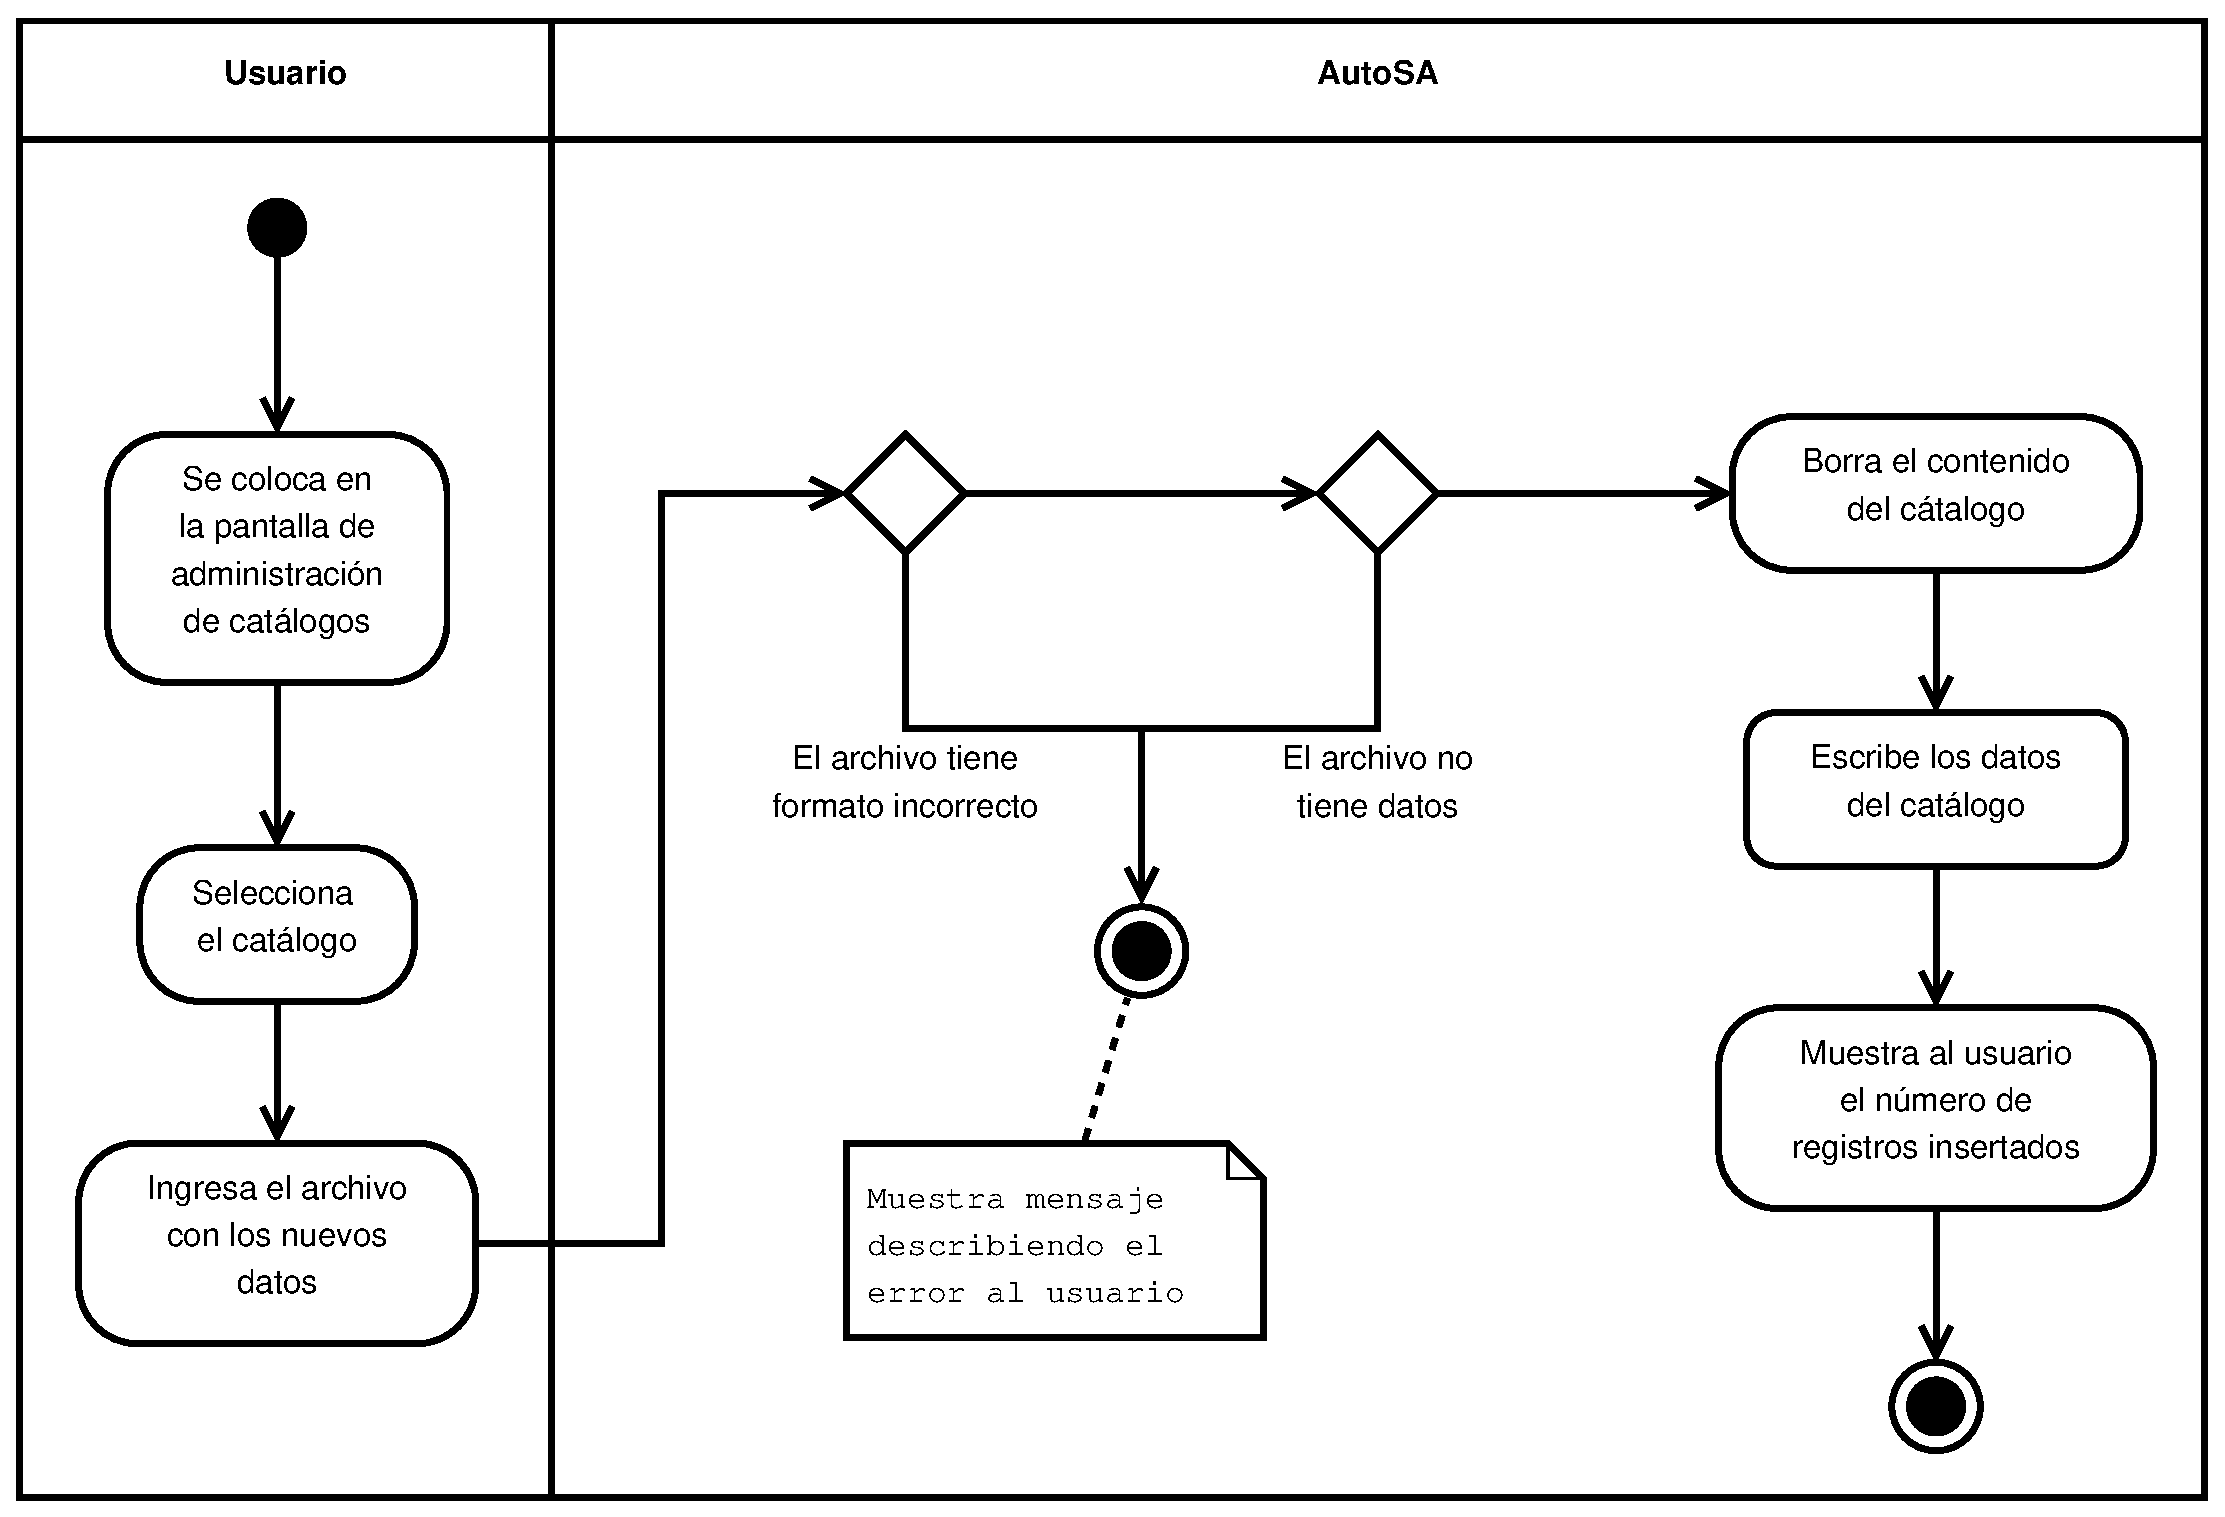
\includegraphics[width=\textwidth]{dia-activity-cat-update}
  \caption{Diagrama de actividad del flujo para la actualización de catálogos.}
  \label{fig:dia-activity-cat-update}
\end{figure}
\paragraph{Precondiciones:}
\begin{enumerate}
  \item El usuario ha iniciado sesión correctamente en la interfaz web (ver caso de uso \textbf{CU-ENTRAR-WEB}).
  \item El archivo ingresado tiene formato extendido de Excel.
  \item Los catálogos que pueden ser modificados por este caso de uso son aquellos que contienen códigos de medicamentos y lugares de entrega.
\end{enumerate}
\paragraph{Secuencia normal:}
\begin{enumerate}
  \item El usuario navega a la pantalla de administración de catálogos.
  \item El usuario realiza las siguientes acciones en la pantalla de administración de catálogos:
  \begin{enumerate}
    \item Seleccionar el nombre del catálogo.
    \item Seleccionar el archivo en formato de Excel que contiene la información para el catálogo.
    \item Enviar el formulario.
  \end{enumerate}
  \item El sistema sigue los siguientes pasos:
  \begin{enumerate}
    \item Valida el formato del archivo recibido.
    \item Valida que el archivo recibido contenga al menos un renglón sin contar el encabezado.
    \item Borra el contenido del catálogo en la base datos y copia la información del archivo recibido.
    \item Muestra al usuario el número de registros guardados en el catálogo después de la actualización.
  \end{enumerate}
\end{enumerate}
\paragraph{Postcondiciones:}
\begin{enumerate}
  \item El catálogo ha sido actualizado al contenido del archivo proporcionado por el usuario.
\end{enumerate}
\paragraph{Excepciones:}
\begin{enumerate}
  \item Si el archivo no cuanta con el formato solicitado, entonces se muestra un mensaje de error al usuario y se cancela la ejecución sin modificar el catálogo en la base de datos.
  \item Si el archivo no contiene ningún registro para el catálogo, entonces se muestra un mensaje de error al usuario y se cancela la ejecución sin modificar el catálogo en la base de datos.
\end{enumerate}


\subsection{Buscar órdenes}\label{cu-buscar}
\paragraph{Identificador:}
CU-BUSCAR
\paragraph{Actores:}
Usuario
\paragraph{Descripción:}
Define el flujo para la búsqueda de órdenes de reposición, la Figura \ref{fig:dia-activity-search} muestra el diagrama de actividad para este caso de uso.
\begin{figure}[h]
  \centering
  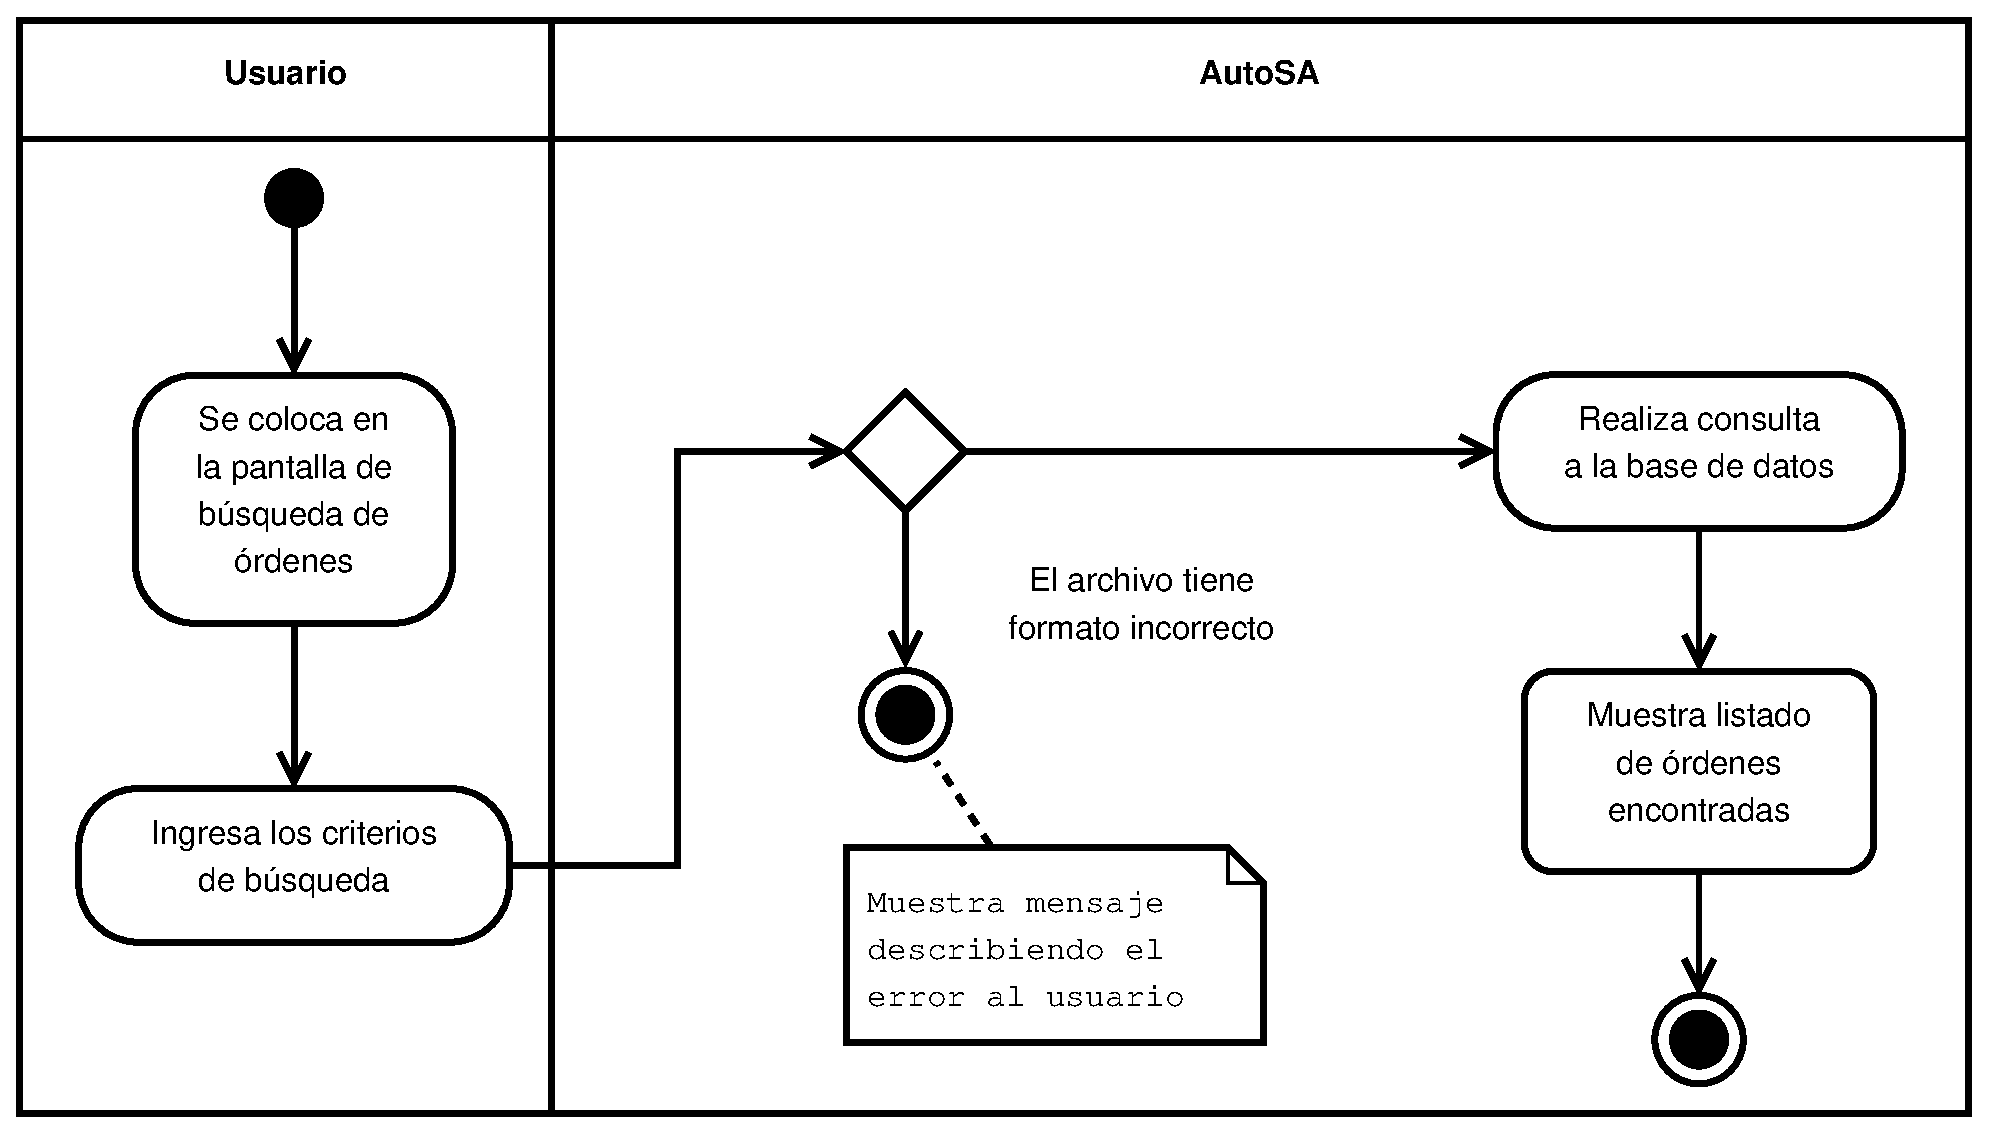
\includegraphics[width=\textwidth]{dia-activity-search}
  \caption{Diagrama de actividad del flujo para la búsqueda de órdenes de reposición.}
  \label{fig:dia-activity-search}
\end{figure}
\paragraph{Precondiciones:}
\begin{enumerate}
  \item El usuario ha iniciado sesión correctamente en la interfaz web (ver caso de uso \textbf{CU-ENTRAR-WEB}).
\end{enumerate}
\paragraph{Secuencia normal:}
\begin{enumerate}
  \item El usuario navega a la pantalla de búsqueda de órdenes de reposición.
  \item El usuario realiza ingresa los criterios para la búsqueda presentados en el filtro:
  \begin{enumerate}
    \item Número de orden.
    \item Estatus de atención.
    \item Rango de fechas en que fueron atendidas las órdenes de reposición.
  \end{enumerate}
  \item El sistema muestra el resultado de la búsqueda, para cada orden de reposición listada se muestra un enlace que lleva a la visualización de la orden (ver casos de uso \textbf{CU-VISUALIZAR}).
\end{enumerate}
\paragraph{Postcondiciones:}
\begin{enumerate}
  \item Se muestra un listado con las órdenes de reposición que cumplen con el filtro definido por el usuario durante el caso de uso.
\end{enumerate}
\paragraph{Excepciones:}
\begin{enumerate}
  \item En caso de no contar con conexión a la base de datos se muestra un mensaje de error informando al usuario.
\end{enumerate}


\subsection{Visualizar orden}\label{cu-visualizar}
\paragraph{Identificador:}
CU-VISUALIZAR
\paragraph{Actores:}
Usuario
\paragraph{Descripción:}
La forma en que el usuario de la interfaz web es capaz de visualizar los datos de una orden de reposición, en la Figura \ref{fig:dia-activity-view} se muestra el diagrama de actividad que sigue este caso de uso, para llegar a esta página es necesario que el usuario haya ejecutado la búsqueda de órdenes de reposición y seleccionado la orden para visualizar como se muestra en la Figura \ref{fig:dia-casos-uso} (ver caso de uso \textbf{CU-BUSCAR}).
\begin{figure}[h]
  \centering
  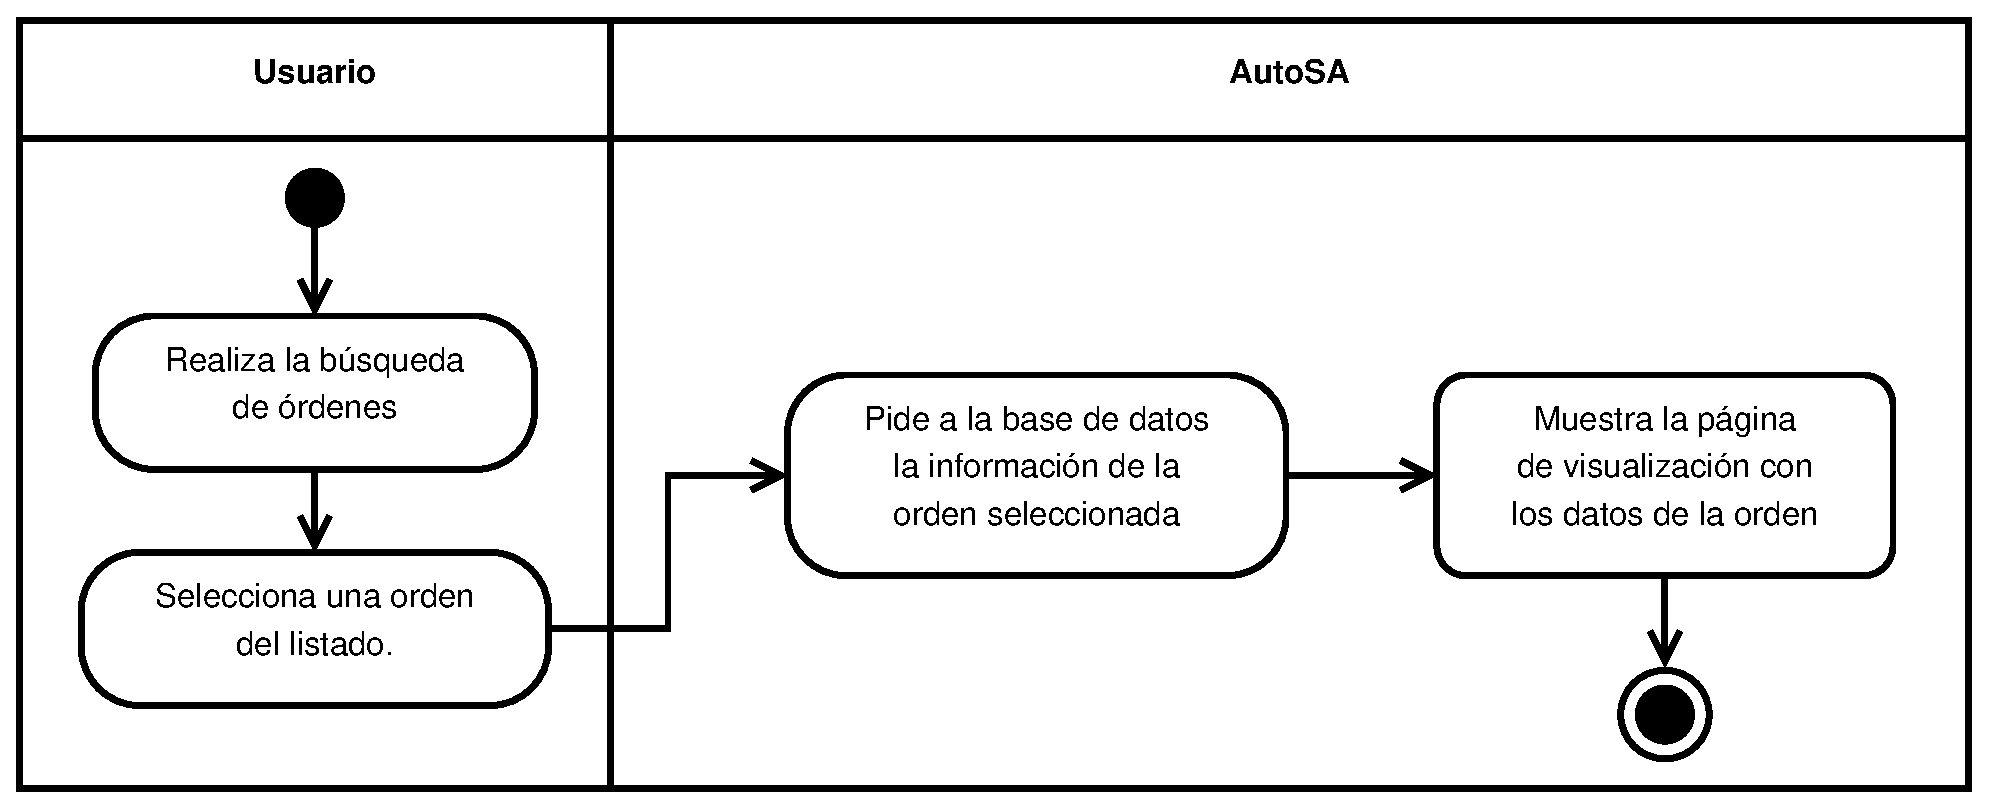
\includegraphics[width=\textwidth]{dia-activity-view}
  \caption{Diagrama de actividad del flujo para la visualización de los datos de una orden de reposición.}
  \label{fig:dia-activity-view}
\end{figure}
\paragraph{Precondiciones:}
\begin{enumerate}
  \item El usuario ha iniciado sesión correctamente en la interfaz web (ver caso de uso \textbf{CU-ENTRAR-WEB}).
  \item El usuario localiza la orden de reposición que desea visualizar (ver caso de uso \textbf{CU-BUSCAR})
\end{enumerate}
\paragraph{Secuencia normal:}
\begin{enumerate}
  \item El usuario navega a la pantalla de visualización de la orden de reposición seleccionada (ver caso de uso \textbf{CU-BUSCAR}).
  \item Se muestra la pantalla con los datos de la orden:
  \begin{enumerate}
    \item Se muestran todos los datos capturados del Sistema de Abastecimiento durante el procedimiento de atención.
    \item También se muestran los estados de atención, es decir el estado en el Sistema de Abastecimiento  y el estado de atención.
  \end{enumerate}
  \item Se muestran enlaces para que el usuario pueda editar los datos de la orden (ver caso de uso \textbf{CU-EDITAR}) y también para generar el acuse de envío (ver caso de uso \textbf{CU-GENERAR-ACUSE}).
  \item En caso de seleccionar la generación del acuse de envío se ejecuta el caso de uso \textbf{CU-GENERAR-ACUSE}.
\end{enumerate}
\paragraph{Postcondiciones:}
\begin{enumerate}
  \item Se muestra una pantalla al usuario con los datos de la orden de reposición solicitada, además las opciones para editar y generar el acuse de envío.
\end{enumerate}
\paragraph{Excepciones:}
\begin{enumerate}
  \item En caso de no contar con conexión a la base de datos se muestra un mensaje de error informando al usuario.
\end{enumerate}


\subsection{Editar orden}\label{cu-editar}
\paragraph{Identificador:}
CU-EDITAR
\paragraph{Actores:}
Usuario
\paragraph{Descripción:}
La forma en que el usuario de la interfaz web puede modificar los datos de una orden de reposición que está visualizando, en la Figura \ref{fig:dia-activity-edit} se muestra el diagrama de actividad que sigue este caso de uso, para llegar a esta vista es necesario que el usuario haya ejecutado la visualización de la orden de reposición que desea modificar. La dependencia de este caso de uso se muestra en la Figura \ref{fig:dia-casos-uso} (ver caso de uso \textbf{CU-BUSCAR}).
\begin{figure}[h]
  \centering
  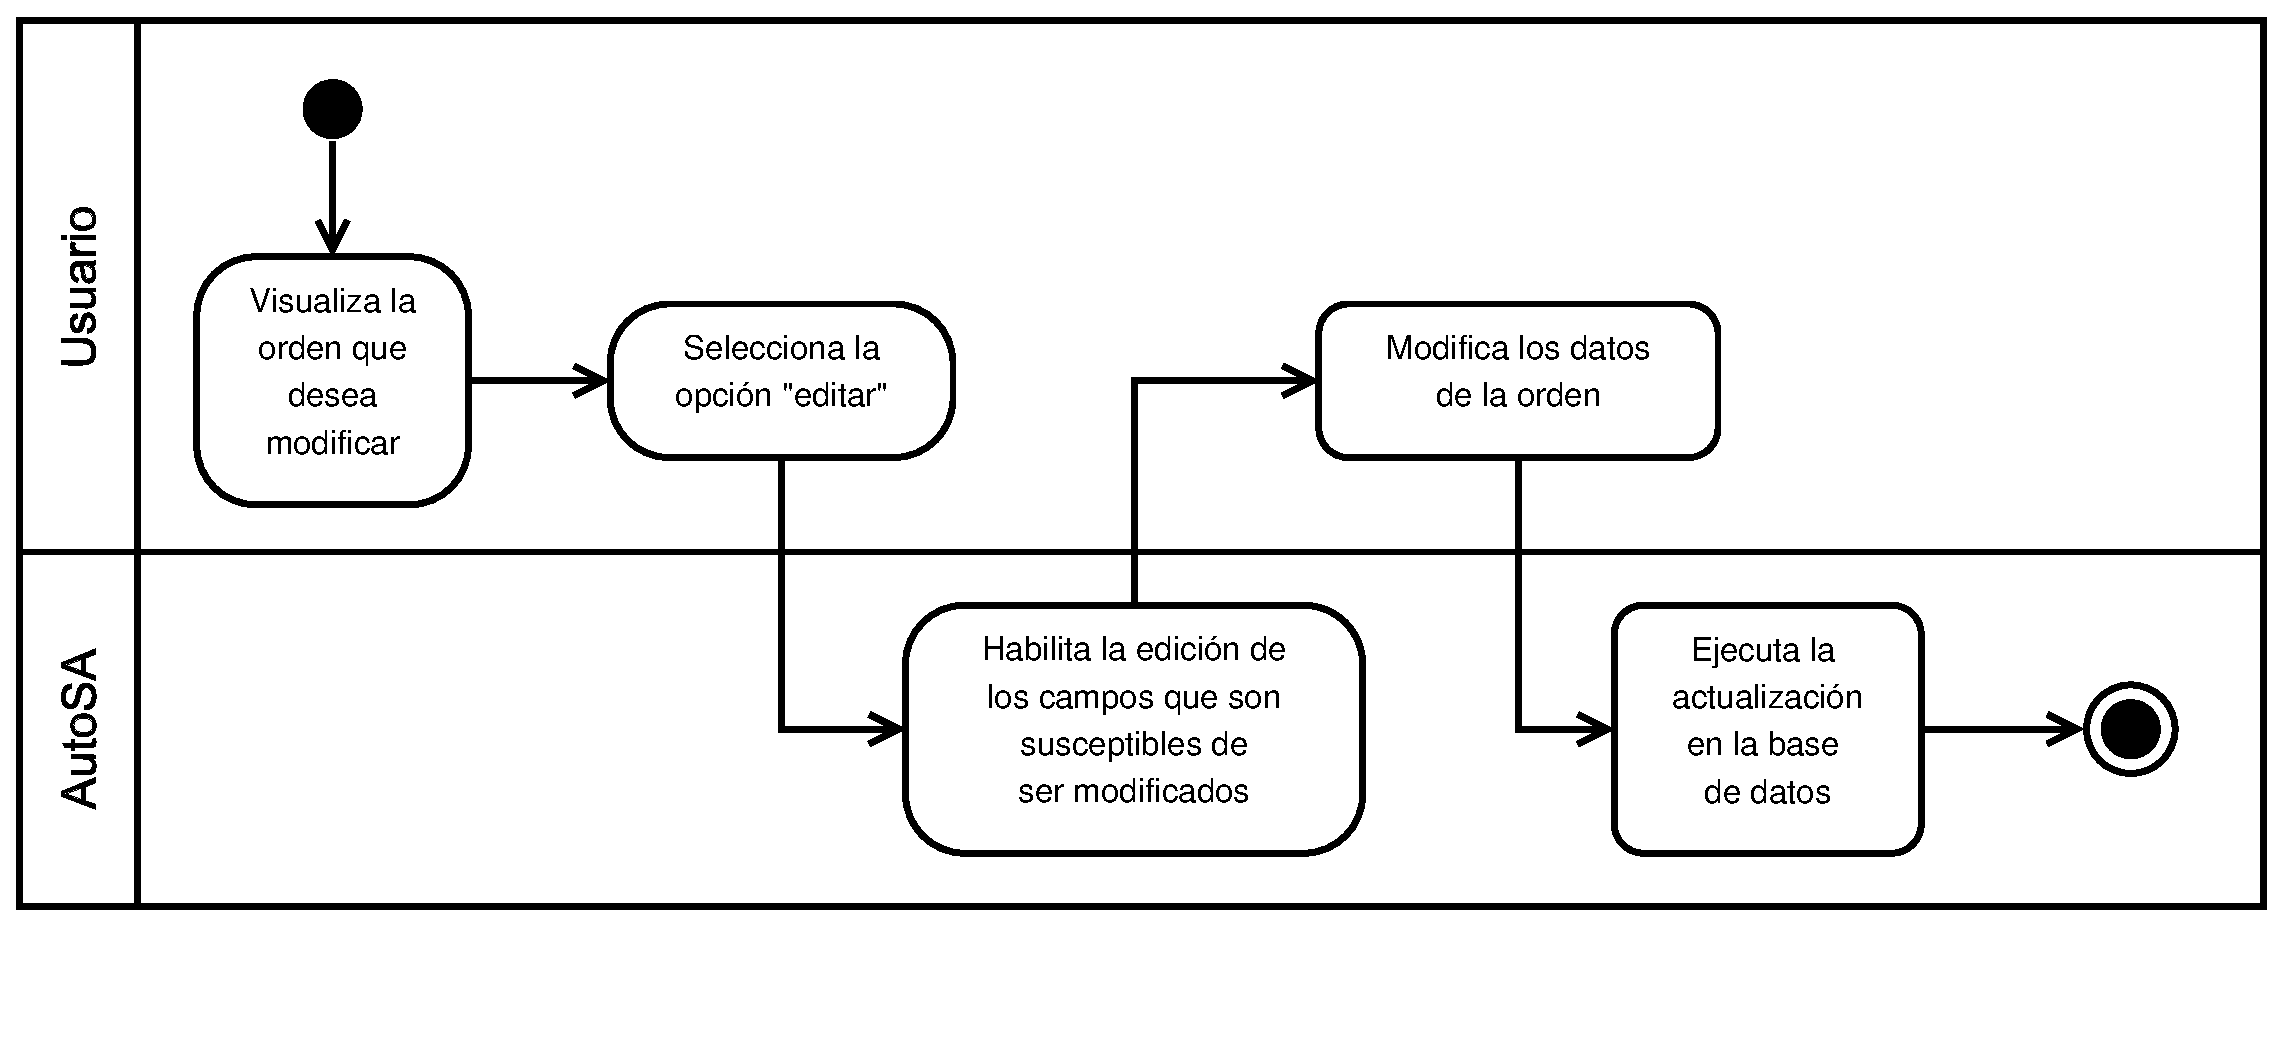
\includegraphics[width=\textwidth]{dia-activity-edit}
  \caption{Diagrama de actividad del flujo para la modificar de los datos de una orden de reposición.}
  \label{fig:dia-activity-edit}
\end{figure}
\paragraph{Precondiciones:}
\begin{enumerate}
  \item El usuario ha iniciado sesión correctamente en la interfaz web (ver caso de uso \textbf{CU-ENTRAR-WEB}).
  \item El usuario visualiza la orden de reposición que desea editar (ver caso de uso \textbf{CU-VISUALIZAR}).
  \item Los campos utilizados para identificar unívocamente la orden de reposición no podrán ser modificados. 
\end{enumerate}
\paragraph{Secuencia normal:}
\begin{enumerate}
  \item El usuario navega a la pantalla de edición con la orden de reposición visualizada (ver caso de uso \textbf{CU-VISUALIZAR}).
  \item Modificar cualquiera de los campos editables.
  \item Seleccionar el botón Guardar.
\end{enumerate}
\paragraph{Postcondiciones:}
\begin{enumerate}
  \item Los datos modificados por el usuario en la interfaz web se encuentran almacenados en la base de datos.
\end{enumerate}
\paragraph{Excepciones:}
\begin{enumerate}
  \item En caso de no contar con conexión a la base de datos se muestra un mensaje de error informando al usuario.
\end{enumerate}
